\chapter{绪论}

\section{研究背景与意义}

水稻（\textit{Oryza sativa}）是全球粮食系统中最重要的作物之一，也是连接粮食安全、农业生计、土地利用变化和气候影响研究的关键对象。与许多以饲料、工业原料或贸易商品属性为主的作物不同，水稻在亚洲、非洲部分地区以及拉丁美洲若干国家直接承担着基础膳食供给功能，其产量波动和区域供给稳定性会迅速传导至居民食物可及性、粮价稳定和农户收入安全。全球人口增长、城市化推进和膳食结构变化持续增加粮食系统压力，而水稻主产区又高度集中于人口密集、季风气候显著且农业劳动力参与度较高的地区，因此水稻生产能力不仅是农业生产问题，也是区域社会经济稳定和粮食安全治理的重要基础\cite{Godfray2010,GRiSP2013,Yuan2021RiceBowl}。在许多发展中国家，水稻种植还与小农经营、灌溉工程维护、农村就业和地方粮食储备制度密切相关，稻田面积和产量的变化往往意味着农户生计结构、农业投入成本和区域粮食自给能力的同步变化。

水稻生产的全球意义并不止于“提供粮食”。稻田是一类高度依赖水热资源和人为管理的农田生态系统，其形成、维持和变化都受到水资源供给、灌溉基础设施、田间水分管理、品种熟期、播栽方式和复种制度的共同控制。与典型旱地作物相比，稻田通常具有阶段性或长期水层覆盖，田面水、土壤背景和水稻冠层共同构成特殊的水—植被复合下垫面。灌溉、排水、移栽或直播、施肥、轮作和休耕等管理行为不仅决定水稻产量，也深刻改变水文过程、土壤氧化还原环境和地表能量交换过程。因此，稻田不能简单视为普通耕地上的一种作物，而应被理解为由水分条件、农田工程和人为管理共同塑造的土地系统单元。已有研究表明，全球耕地扩张、农业集约化和水资源管理正在重塑陆地生态系统格局，并对生物多样性、水文循环和区域环境产生深远影响\cite{Foley2005,Potapov2022,Zabel2019,McDermid2023Irrigation}；稻田作为高水分需求和强人为调控的农田类型，在这一过程中具有突出的资源和环境指示意义。

由此可见，水稻既是粮食作物，也是重要的环境影响源。水稻生产需要消耗和调配大量农业用水，可能推动灌溉设施扩展、湿地或旱地转换以及局地土地利用变化；稻田淹水环境还会影响土壤碳氮循环和农业温室气体排放。与此同时，土地利用和土地管理并非只通过碳循环影响气候，还会通过反照率、蒸散发、地表粗糙度和热容量等生物物理过程改变地表能量平衡和局地热环境\cite{Bright2017LCMC,Duveiller2018Energy,Chen2024Croplands}。稻田由于同时具有开放水面、湿润土壤和季节性植被冠层，其环境影响天然包含资源消耗、生物地球化学排放和地表生物物理调节等多个维度。因此，研究全球稻田不仅是为了回答“水稻在哪里生产、生产多少”，更是为了理解这一特殊农田系统如何在保障粮食供给的同时影响水资源、土地系统和局地气候。

在稻田环境影响中，气候效应长期以来首先被理解为温室气体排放问题，尤其是甲烷（CH$_4$）排放问题。稻田在长期或阶段性淹水条件下容易形成厌氧土壤环境，促进产甲烷菌活动和有机质厌氧分解，使稻田成为农业甲烷排放的重要来源。围绕这一过程，已有大量研究从稻田土壤生物地球化学机制、区域和全球温室气体清单、水分管理、秸秆还田、施肥制度以及减排措施等方面建立了较为系统的知识框架\cite{Qian2023RiceGHG,Zhang2020NatCommun}。这些研究对于认识水稻生产的气候代价、制定农业减排策略和改进国家温室气体清单具有不可替代的意义，也使“稻田—甲烷—增温”成为稻田气候效应研究中最为熟悉的逻辑链条。

然而，将稻田气候效应仅理解为温室气体增温效应是不完整的。稻田在水稻生长季内通常具有较高的土壤湿度和蒸散发能力，田面水层蒸发与水稻冠层蒸腾共同增强潜热通量，使更多可利用能量以水汽相变的方式释放到大气中，而不是以显热形式直接升高地表温度和近地表空气温度。在净辐射条件相近时，潜热通量的增加通常意味着显热通量的相对减少，从而表现为稻田地表温度（land surface temperature, LST）低于周边非稻田农田。灌溉农田和植被变化研究已经表明，农业水分管理和地表覆盖变化能够显著改变局地地表温度\cite{Thiery2020Irrigation,McDermid2023Irrigation,Chen2024Croplands}；稻田作为典型水—植被复合下垫面，其水分条件和冠层发育过程更可能在水稻生长季内形成具有物候阶段性的地表降温效应。

这种地表生物物理降温效应与温室气体增温效应共同构成稻田气候影响的双重性。一方面，稻田淹水条件会通过甲烷排放参与大气辐射强迫，表现为生物地球化学意义上的气候增温影响；另一方面，稻田水层蒸发和水稻冠层蒸腾又会通过地表能量分配改变LST，表现为局地或区域尺度的地表生物物理降温影响。已有区域尺度研究和近期全球遥感研究均提示，稻田生长季内相较周边非稻田农田可能表现出更低的地表温度，但与稻田甲烷排放相比，稻田地表降温效应在全球尺度上的系统量化和机制认识仍相对不足\cite{Xue2021RemoteSensing,Weng2025}。这并不意味着应将稻田视为“有益降温源”而忽略其排放风险，而是说明稻田气候效应本身具有多过程、多尺度和多指标的复杂属性。

因此，当前稻田气候效应研究面临一个需要澄清的认识偏差：如果只从甲烷排放理解稻田，就会低估或忽略稻田通过地表能量平衡调节局地热环境的作用；如果只强调稻田降温，又可能弱化其温室气体排放带来的全球气候风险。更严谨的认识是，稻田地表降温效应补充了现有对稻田气候效应的理解，但它与温室气体增温效应属于不同过程、不同尺度和不同指标，不能直接等量抵消。温室气体排放主要作用于大气成分和辐射强迫，具有长期累积和全球混合特征；地表生物物理降温主要通过蒸散发、显热通量和地表能量分配影响LST，具有更强的局地性、季节性和下垫面依赖性。只有同时区分并联系这两个维度，才能形成对稻田气候效应更加完整而不失严谨的综合认识。

要从综合视角评估水稻生产的环境影响，尤其是评估稻田地表生物物理降温效应，首先需要可靠回答一组基础问题：稻田在哪里，何时处于水稻生长季，生长季持续多久，在景观中以何种斑块规模和空间结构存在。水稻时空动态信息并不只服务于地表温度研究，也支撑粮食安全评估、水资源利用核算、土地利用变化监测、温室气体排放估算和农业气候影响评估。稻田面积决定环境效应发生的空间范围，生长季决定蒸散发、甲烷排放和LST响应的时间窗口，空间结构则决定稻田与周边非稻田农田之间的热环境对比和潜在外溢影响。缺乏一致、连续且具有生长季信息的水稻数据，环境效应评估就容易受到空间范围误判、时间窗口错配和区域可比性不足的影响。

全球覆盖是稻田环境影响评估的首要数据需求。稻田降温效应并不是某一个国家或某一类稻区的局地问题。亚洲是全球水稻生产的核心区域，但非洲、美洲、欧洲和大洋洲均分布有具有代表性的稻作系统；这些区域在气候背景、灌溉条件、地形地貌、田块形态、作物制度和农田管理方面差异显著。热带湿润区可能存在多季稻和高度灵活的播栽安排，温带稻区通常受温度季节性约束而以单季稻为主，半干旱灌溉稻区则可能表现出更强的水分管理效应。若仅依赖中国、东南亚、美国或日本等局部区域数据，很难判断稻田地表降温是否具有全球普遍性，也无法比较不同洲、不同气候区和不同种植制度下的效应差异。因此，全球一致的水稻种植区数据是将稻田降温效应从区域现象提升为全球土地系统问题的基本前提。

空间分辨率决定了稻田空间结构和局地热环境差异能否被表达。传统统计分配型或粗分辨率全球作物产品适用于宏观面积统计、粮食安全模型和水文模拟，但其像元尺度往往难以刻画稻田与周边非稻田农田之间的空间邻近关系，也难以支持田块规模、稻田比例、景观破碎度和外溢降温效应分析。已有全球作物数据集，如Monfreda等构建的全球作物面积与产量格局、MIRCA2000、GAEZ+\_2015、CROPGRIDS和GloRice等，为全球农业模型和长期面积分析提供了重要基础\cite{Monfreda2008CropDistribution,Portmann2010MIRCA,Grogan2022GAEZ,Tang2024CROPGRIDS,Xie2025GloRice}。但对于稻田地表降温效应研究而言，仅有粗分辨率面积比例仍不足以描述稻田斑块与邻近农田之间的热环境关系。相较多数粗分辨率全球产品明显提高的中等空间分辨率水稻数据，能够在全球尺度上更细致地刻画稻田空间异质性，为分析稻田斑块规模、稻田比例及其对LST的影响提供必要基础。需要特别强调的是，500 m不宜称为严格意义上的高空间分辨率；其意义在于在全球覆盖、长期连续、较细空间表达和可计算性之间形成可行平衡。

长期连续信息是理解全球稻田环境效应变化的另一项关键需求。稻田面积和空间格局并非固定不变，而是随着人口需求、粮食价格、农业政策、城市化、水资源约束和灌溉工程建设不断调整。21世纪以来，全球耕地扩张和农业集约化在不同区域呈现显著差异\cite{Potapov2022,Zabel2019}，稻田也可能出现非洲部分地区快速扩张、美洲部分稻区收缩、亚洲内部种植重心转移等过程。这些变化会改变水资源利用、温室气体排放和地表降温效应的空间贡献。如果只有某一年或少数年份数据，研究只能获得静态快照，无法回答全球稻田面积是否持续扩张、稻田降温效应是否随时间变化、哪些区域对全球效应的贡献增加或减少，以及多年平均降温效应是否稳定等问题。长期连续水稻数据能够降低单一年份气候异常、种植波动或遥感观测噪声带来的不确定性，是开展多年尺度环境效应估计和趋势分析的基础。

高时间分辨率则直接决定稻田气候效应评估的时间匹配精度。只知道年度稻田空间分布是不够的，因为稻田地表降温效应主要发生在水稻生长季内，并且其强度随水层状态、冠层发育和蒸散发过程而变化。年度土地覆盖图无法判断某个稻田像元在特定日期是否处于移栽期、旺盛生长期、成熟期或收获后阶段，也难以识别热带和亚热带地区常见的双季稻、多季稻或错季种植。日尺度或近似日尺度的水稻生长季信息能够支持水稻生长季开始时间（start of season, SOS）、结束时间（end of season, EOS）、生长季长度和复种制度识别，从而为LST分析提供真实的时间窗口。若采用固定月份计算稻田与非稻田农田的LST差异，很容易将非生长季、休耕期、轮作作物期或错季水稻纳入分析，尤其在热带多熟区，水稻生长月份并不固定，固定时间窗会造成系统性时间错配。只有准确识别水稻生长季起止时间，才能将观测到的LST差异与水稻生长和稻田水分蒸散过程建立可靠联系。

综合来看，全球水稻时空动态数据需要同时具备全球覆盖、相较粗分辨率产品更高的空间分辨率、长期连续和高时间分辨率等特征。现有全球或大尺度水稻数据产品往往只能满足其中部分需求：统计分配型产品具有全球覆盖和长期序列优势，但空间细节和生长季过程不足；区域遥感产品空间分辨率较高，但难以支撑全球一致分析；部分全球水稻产品能够用于面积统计，却缺少逐像元、逐日或生长季尺度的动态信息\cite{Dong2016,Xiao2006,Xie2025GloRice}。因此，构建全球水稻时空动态数据集并非单纯的数据生产任务，而是开展水稻环境影响与稻田地表气候效应评估的关键前提。对于稻田降温效应而言，水稻数据集的价值不仅在于划定稻田范围，更在于为“何时比较LST”“与哪些周边农田比较”“如何解释空间结构差异”提供一致的时空基础。

然而，全球水稻动态制图本身面临显著复杂性。首先，稻田下垫面不同于普通旱地作物，其遥感信号来自水层、土壤背景和植被冠层的共同作用。在移栽或返青阶段，浅水覆盖和稀疏植被可能同时存在，光学遥感观测常表现为较强水分信号和较低植被指数；随后水稻冠层快速生长，植被指数升高，水面信号逐渐被冠层遮蔽；成熟和收获后，植被指数迅速下降，土壤、水分和残茬背景再次影响像元光谱。合成孔径雷达观测也会受到水层、植株结构、冠层高度和田间粗糙度变化的共同影响。正是这种水文过程与植被过程耦合、且主导信号随生育阶段转换的特征，使稻田遥感时序明显区别于多数旱地作物\cite{Dong2016,Zhan2021}。

其次，稻田高度受人为管理影响，其时序特征并不完全遵循自然植被那样相对稳定的季节节律。播栽期可以因灌溉供水、季风降雨开始时间、劳动力安排、品种熟期和市场需求而改变；直播和移栽会形成不同的早期水分与植被信号；连续淹水、间歇灌溉和雨养水稻会改变水层可见性和土壤湿度；轮作、休耕、再生稻以及双季或多季种植会使同一像元在一年内出现多个持续时间不同的生长周期。这些管理差异不仅影响稻田是否能够被识别，也影响SOS、EOS和生长季长度的确定。稻田因此不是具有固定物候模板的静态土地覆盖类型，而是受农户决策、灌溉制度、地方政策和区域农业经济共同调控的生产系统。

再次，全球稻区差异显著，使局部经验难以直接推广。温带地区水稻通常受热量条件限制，以单季稻为主，播栽和收获时间具有较明确的季节边界；亚热带季风区可能存在早稻、晚稻、稻—麦或稻—油等轮作制度；热带地区水热条件相对充足，播种时间不受固定季节严格约束，双季稻、多季稻和错季种植均可能存在，生长季不确定性更强。除气候条件外，水资源可得性、地形、田块大小、劳动力成本、机械化水平、农业政策和地方种植习惯也会改变水稻种植制度。全球水稻动态制图的难点因此不只是提高分类精度，而是要在不同气候区、不同种植制度和不同管理方式下稳定识别稻田真实生长季。

这些复杂性决定了全球水稻制图不能简单依赖固定时间窗、固定阈值或局部区域经验。基于物候和淹水先验的方法具有明确物理意义，但在旱直播、间歇灌溉、弱淹水信号和复杂复种制度下容易出现漏分或错分；机器学习和深度学习方法能够融合多源特征并在样本充足的区域取得较高精度，但其跨区域、跨年份泛化能力仍受到训练样本、作物制度差异和观测条件变化的限制\cite{Zhao2024OpticalRadar}；基于时间序列相似性的曲线匹配方法能够适应一定程度的物候相位差异，但仍需要解决不同生长季长度、重复种植周期以及非水稻湿地或水体混淆等问题。因此，面向全球应用的水稻动态制图方法需要同时具备物候可解释性、时序弹性和跨区域稳定性，能够从“识别某一年某一区域的水稻分布”进一步发展为“稳定刻画全球稻田何时生长、持续多久以及如何变化”的动态监测框架。

基于上述背景，开展全球水稻时空格局遥感监测及其地表降温效应研究具有明确的科学认识意义。它有助于补充稻田气候效应中长期相对薄弱的地表生物物理降温维度，推动稻田气候影响研究从“温室气体排放单一视角”走向“生物地球化学过程+地表生物物理过程”的综合认识。这样的综合认识并不意味着将甲烷增温效应与LST降温效应作简单抵消，而是将不同尺度、不同过程和不同指标的气候影响放在同一土地系统框架下加以区分和理解。对于农业遥感和土地系统科学而言，这一视角能够把作物分布、物候过程、农田水分管理和地表能量平衡联系起来，从而更完整地解释水稻生产系统在全球变化背景下的环境角色。

本研究还具有重要的方法与数据意义。发展全球适用的水稻动态制图方法，构建长期、日尺度、中等空间分辨率的全球水稻数据集，可以为全球农业遥感、作物物候监测、土地系统变化和水稻环境影响评估提供基础数据支撑。相比只回答“哪里是稻田”的年度静态制图，水稻动态制图进一步关注“稻田何时生长、持续多久、是否存在多季种植以及空间结构如何变化”。这些信息能够把作物遥感制图与生态过程评估连接起来，使水稻面积、物候、景观格局、蒸散发和LST分析具有一致的时空边界。换言之，全球水稻动态数据集不仅是制图成果，也是连接粮食安全、水资源、温室气体排放和地表气候效应研究的基础设施。

从应用角度看，全球水稻时空动态数据和稻田地表降温效应评估能够服务于多类现实需求。对于粮食安全评估，它可以揭示全球水稻种植区扩张、收缩和区域转移，为识别供给风险和生产潜力提供依据；对于农业资源管理和水资源利用评估，它可以帮助刻画稻田灌溉需求和生长季水分消耗的时空范围；对于区域热环境和气候适应型农业管理，它可以为认识稻田在农田生态系统热调节中的作用提供证据。更广泛地说，在全球变暖、极端高温风险上升和农业可持续转型并行的背景下，系统刻画全球稻田分布、生长季动态及其地表生物物理效应，有助于为兼顾粮食安全、资源利用效率和农田生态系统气候调节功能的农业管理提供科学依据。

\section{全球水稻遥感制图研究进展}

全球水稻遥感制图是开展稻田时空动态监测与环境效应评估的基础。近二十年来，随着卫星遥感技术、云计算平台和人工智能方法的快速发展，全球或大区域水稻数据产品的空间分辨率和时间覆盖能力持续提升，水稻识别方法也从简单阈值判断演进到复杂的时间序列分析与深度学习分类\cite{Dong2016}。然而，正如1.1节所述，全球水稻动态制图在对象复杂性、数据产品供给和方法综合能力等方面仍面临显著瓶颈。本节从数据产品和方法论两个维度系统梳理已有研究进展，厘清全球水稻制图领域已解决与尚未解决的关键问题，为后文第三章和第四章的方法构建与数据集开发奠定文献基础。

\subsection{全球水稻数据集发展现状}

全球水稻空间数据的发展经历了从统计资料空间化到遥感直接识别的演变。早期产品以农业统计为基础，通过空间分配模型实现全球覆盖；近年来，中高分辨率遥感数据的应用使稻田边界识别和空间格局刻画能力显著提升。然而，不同数据产品在空间分辨率、时间分辨率、时间覆盖和生长季信息之间存在明显权衡，尚无产品能够同时满足全球稻田环境效应评估的全部数据需求。以下从统计分配型数据集、遥感识别型数据集和数据集发展趋势三个层面加以梳理。

\subsubsection{基于统计资料和空间分配模型的全球水稻/作物数据集}

早期全球水稻空间数据主要来源于统计资料与空间分配模型的融合。20世纪末至21世纪初，随着联合国粮农组织（FAO）全球农业统计数据库的完善和GIS空间分析技术的发展，研究者开始将国家或次国家尺度的作物面积、产量统计数据与耕地分布、作物历、灌溉信息、气候适宜性或土地覆盖数据相结合，通过空间分配模型生成全球一致的作物栅格数据。这类方法的基本逻辑是：先确定某行政单元内某种作物的总面积，再依据该单元内的耕地分布、灌溉可达性、农业适宜性或已有作物分布先验，将统计面积分配至栅格像元\cite{Leff2004,Monfreda2008CropDistribution}。

这类数据集的优势在于全球覆盖、变量体系相对完整，并且能够与农业统计口径保持较好衔接，便于与宏观经济模型、粮食安全评估框架和全球水文模型对接。例如，Leff等研制的全球作物分布图较早系统刻画了主要作物类型的全球空间格局\cite{Leff2004}；Monfreda等进一步在2000年基准年上提供了全球作物面积、产量和净初级生产力的1 km分辨率栅格数据，成为此后十余年农业地理学和全球变化研究的重要基础\cite{Monfreda2008CropDistribution}。在此基础上，MIRCA2000将作物分布与灌溉、雨养信息相结合，提供了全球月度作物物理面积数据，支撑了大量农业水文和作物模型研究\cite{Portmann2010MIRCA}。近年来，GAEZ+\_2015和CROPGRIDS等产品进一步更新了作物分布数据的时间覆盖和变量体系，为全球农业变化监测提供了更为丰富的数据选择\cite{Grogan2022GAEZ,Tang2024CROPGRIDS}。

然而，统计分配型数据集的本质局限在于其空间分辨率较粗且缺少遥感直接识别意义上的稻田边界和时序动态信息。上述产品的空间分辨率多为5 arc-min、10 km或0.5$^\circ$等较粗尺度，且不少产品仅代表某一年或少数基准年，难以反映田块尺度稻田边界、景观破碎化格局和年际变化过程。对于需要回答"稻田在哪里""稻田何时处于生长季"以及"稻田与周边农田的空间关系如何"等问题的研究而言，统计分配型产品通常只能提供面积或比例信息，无法刻画水稻种植过程的时序动态，也难以支撑基于遥感观测的稻田斑块结构和局地环境效应分析。

长时序全球水稻面积数据仍具有不可替代的宏观分析价值。例如，GloRice v1.0基于FAO统计资料和空间分配模型，提供了1961--2021年5 arc-min全球水稻收获面积和物理面积数据，时间跨度超过六十年，适合用于长时间尺度农业变化趋势分析、粮食安全统计研究和全球农业政策评估\cite{Xie2025GloRice}。类似地，SPAM系列产品通过融合统计数据与多种空间协变量，提供了全球多种作物的收获面积、产量和价值分布，在农业经济和水资源研究中得到广泛应用。但由于空间分辨率较粗，且缺少像元级物候信息，这类数据仍难以支撑精细尺度稻田格局刻画、生长季过程追踪和稻田环境效应的动态研究。换言之，统计分配型产品回答了"某区域有多少水稻"的问题，却难以回答"具体像元是否为稻田、何时开始生长、持续多久"的问题。

\subsubsection{基于遥感识别的大区域水稻数据集}

近年来，随着中高分辨率卫星观测能力的提升和云计算平台（如Google Earth Engine）的普及，学界开始研制更明确的遥感识别型大尺度水稻产品。与统计分配型数据相比，这类产品直接利用光学、合成孔径雷达（SAR）或多源遥感时间序列识别稻田，空间分辨率更高，能够更好地刻画稻田边界、空间聚集格局和区域扩张收缩过程。遥感识别型产品的出现标志着全球水稻数据从"统计推算"走向"遥感观测"的重要转折。

在亚洲主产区，已有研究构建了中国、印度、东北亚、东南亚等区域的长时序或高分辨率稻田分布图，部分产品空间分辨率已达到10--30 m，为区域尺度水稻面积估算、种植制度识别和管理决策提供了重要支撑。例如，Zhang等基于Landsat时间序列和决策树方法研制了中国和印度2000--2015年500 m分辨率水稻分布图，揭示了两大产稻国水稻面积的空间格局与变化趋势\cite{Zhang2017STOTEN}；Han等基于Sentinel-2和Landsat数据构建了2017--2019年东北亚和东南亚10 m分辨率年度水稻图（NESEA-Rice10），显著提升了稻田边界刻画精度\cite{Han2021}；Gumma等利用MODIS 500 m数据在孟加拉国高复种强度环境下实现了季节性水稻面积提取，展示了中等分辨率数据在复杂种植制度区的应用潜力\cite{Gumma2014}。此外，基于Sentinel-1 SAR时间序列的研究在缅甸等云雨频发区取得了重要进展，证明了雷达数据在克服光学遥感云覆盖限制方面的独特价值\cite{Torbick2017}。这些区域产品的共同特点是空间分辨率较高、遥感识别属性明确，能够为区域农业管理和精准农业应用提供较精细的空间信息。

然而，遥感识别型产品的快速发展并未从根本上解决全球一致性和长期连续性问题。现有高分辨率水稻图多集中于亚洲主产区或少数国家，空间覆盖范围有限，难以支撑全球一致分析；一些全球或近全球产品虽然覆盖范围更广，但往往缺少长期连续序列或逐日生长季信息，难以用于年际变化分析和多年平均环境效应评估。特别是在热带多熟区、云雨频发区和小农经营导致的破碎化稻区，单一传感器和单一年份产品仍难稳定反映复杂的水稻种植动态。此外，不同区域产品采用的遥感数据源、分类方法、验证策略和产品格式各不相同，导致产品之间缺乏可比性和可拼接性，限制了它们在更大空间尺度上的综合应用。

\subsubsection{全球水稻动态数据集的发展趋势与局限}

综合来看，现有全球水稻产品在空间分辨率、时间分辨率、时间覆盖、生长季信息和全球适用性之间存在明显权衡（表~\ref{tab:rice_products}）。统计分配型产品实现了长时序全球覆盖，但空间和时间分辨率较粗，缺乏遥感识别意义上的稻田边界和像元级动态信息；遥感识别型产品提升了空间细节，却往往局限于区域尺度或少数年份，难以提供长期、连续和像元级的动态生长季信息。这种"时空权衡"并非偶然的技术局限，而是由不同数据产品的设计目标、数据源特性和生产约束共同决定的：统计分配型产品服务于宏观农业分析和经济模型，遥感识别型产品服务于区域农业监测和精准管理，二者的功能定位本就不同。

\begingroup
\footnotesize
\setlength{\tabcolsep}{3pt}
\setlength{\LTleft}{0pt}
\setlength{\LTright}{0pt}
\begin{longtable}{@{}>{\raggedright\arraybackslash}p{0.28\textwidth}>{\raggedright\arraybackslash}p{0.11\textwidth}>{\raggedright\arraybackslash}p{0.15\textwidth}>{\raggedright\arraybackslash}p{0.17\textwidth}>{\raggedright\arraybackslash}p{0.11\textwidth}>{\raggedright\arraybackslash}p{0.11\textwidth}@{}}
\caption{典型全球及大区域水稻/作物数据集主要特征对比}
\label{tab:rice_products}\\
\toprule
产品名称 & 应用类型 & 覆盖范围 & 时间范围 & 空间分辨率 & 发布时间 \\
\midrule
\endfirsthead
\toprule
产品名称 & 应用类型 & 覆盖范围 & 时间范围 & 空间分辨率 & 发布时间 \\
\midrule
\endhead
\bottomrule
\endfoot
% Cropland Data Layer (CDL)\cite{Boryan2011CDL} & 作物类型 & 美国本土 & 2008年至今 & 30 m & 正在更新 \\
% Cropland Data Layer (CDL)\cite{Boryan2011CDL} & 作物类型 & 部分美国本土 & 1997--2007年 & 30 m & 正在更新 \\
\multirow[t]{2}{=}{Cropland Data Layer (CDL)\cite{Boryan2011CDL}} 
& \multirow[t]{2}{=}{作物类型} 
& 美国本土 
& 2008年至今 
& \multirow[t]{2}{=}{30 m} 
& \multirow[t]{2}{=}{正在更新} \\

& 
& 部分美国本土 
& 1997--2007年 
& 
& \\
CROPGRIDS\cite{Tang2024CROPGRIDS} & 作物类型 & 全球 & 2020年 & $0.05^\circ$ & 2024年 \\
GEOGLAM-BACS v.1.0\cite{BeckerReshef2023GEOGLAMBACS} & 作物类型 & 全球 & 未说明 & $0.05^\circ$ & 2023年 \\
东南亚20 m年度水稻分布图\cite{Sun2023SEAsiaRice20m} & 水稻分布 & 东南亚 & 2019年 & 20 m & 2023年 \\
南亚水稻产量降尺度图\cite{Mohanasundaram2023SouthAsiaYield} & 水稻产量 & 南亚 & 2000--2015年 & 500 m & 2023年 \\
韩国动态水稻分布图\cite{Jo2023KoreaDynamicRice} & 水稻分布 & 韩国 & 2017--2021年 & 10 m & 2023年 \\
GAEZ+\_2015\cite{Grogan2022GAEZ} & 作物类型 & 全球 & \makecell[l]{2015年\\（月度）} & 5 arc-min & 2022年 \\
日本历史水稻田分布图\cite{Carrasco2022JapanRice} & 水稻分布 & 日本（不含冲绳） & \makecell[l]{1985--2019年\\（5年合成）} & 30 m & 2022年 \\
亚洲季风区水稻数据集\cite{Han2022AsianMonsoonRice} &  \makecell[l]{水稻分布/\\复种强度} & 亚洲季风区 & 2000--2020年 & 500 m & 2022年 \\
NESEA-Rice10\cite{Han2021} & 水稻分布 & 东北亚、东南亚 & 2017--2019年 & 10 m & 2021年 \\
RLCMS\cite{RLCMS} & 作物类型 & 东南亚 & 2000年至今 & 30 m & 正在更新 \\
日本Sentinel-1/2水稻图\cite{Inoue2020JapanPaddy} & 水稻分布 & 日本 & 2018年 & 30 m & 2020年 \\
ChinaCropPhen1km\cite{Luo2020ChinaCropPhen} & 作物物候 & 中国 & 2000--2015年 & 1 km & 2020年 \\
中国三大粮食作物收获面积\cite{Luo2020ChinaHarvest} & 作物类型 & 中国 & 2000--2015年 & 1 km & 2020年 \\
GDHY v1.2 + v1.3\cite{Iizumi2020GDHY} & 作物产量 & 全球 & 1981--2016年 & $0.05^\circ$ & 2020年 \\
GDHY v1.2\cite{Iizumi2018GDHY} & 作物产量 & 全球 & 1981--2008年 & $0.05^\circ$ & 2018年 \\
GDHY\cite{Iizumi2014GDHY} & 作物产量 & 全球 & 1982--2006年 & $1.125^\circ$ & 2014年 \\
SPAM V2.0\cite{Yu2020SPAM} &  \makecell[l]{作物类型/\\作物产量} & 全球 & 2010年 & $0.05^\circ$ & 2020年 \\
SPAM\cite{You2014SPAM} & 作物产量 & 全球 & 2000年 & 5 arc-min & 2014年 \\
孟加拉国季节性水稻分布图\cite{Gumma2014} & 水稻分布 & 孟加拉国 & 2010年 & 500 m & 2014年 \\
南亚MODIS水稻分布图\cite{Gumma2011SouthAsiaRice} & 水稻分布 & 南亚 & 2000--2001年 & 500 m & 2011年 \\
尼泊尔水稻种植区变化图\cite{Gumma2011NepalRice} & 水稻分布 & 尼泊尔 & 2000--2009年 & 500 m & 2011年 \\
MIRCA2000\cite{Portmann2010MIRCA} & 作物类型 & 全球 & \makecell[l]{2000年\\（月度）} & 5 arc-min & 2010年 \\
全球作物生产数据\cite{Monfreda2008CropDistribution} & \makecell[l]{作物类型/\\作物产量} & 全球 & 2000年 & 5 arc-min & 2008年 \\
南亚与东南亚MODIS水稻图\cite{Xiao2006} & 水稻分布 & 南亚、东南亚 & 2002年 & 500 m & 2006年 \\
全球主要作物分布图\cite{Leff2004} & 作物类型 & 全球 & 1990年 & 约10 km & 2004年 \\
\end{longtable}
\endgroup

这一局限直接制约了稻田环境效应研究。稻田甲烷排放、水资源消耗、蒸散发过程和地表温度效应均与真实生长季密切相关，如果仅使用年度静态水稻图或固定月份窗口，容易忽略不同区域播栽期、生长季长度和复种制度的差异，进而导致环境效应评估中的时间窗口错配和空间范围误判。例如，在热带多熟区，固定月份可能同时覆盖两季的生长期和休闲期，使得基于该窗口计算的蒸散发或地表温度差异难以准确归因于水稻生长过程；在温带单季稻区，若某年气候异常导致播栽期推迟，固定月份窗口则可能将移栽前的非稻田阶段错误纳入分析。

因此，面向稻田环境效应评估的全球水稻数据集，不应只追求更高空间分辨率，还需要同时兼顾全球覆盖、长期时间覆盖、中等空间分辨率、高时间分辨率和生长季信息。中等空间分辨率（如500 m）的意义并非提供田块尺度的精细边界，而是在全球覆盖、长期连续、较细空间表达和可计算性之间形成可行平衡，使稻田斑块与周边非稻田农田的空间邻近关系得以被刻画，同时保证20年以上全球时间序列的可处理性。日尺度或近似日尺度的生长季信息则能够将环境效应分析的时间基准从"固定月份"提升至"真实生育期"，显著增强效应归因的精确性。现有数据产品往往只能满足上述需求的一部分，这意味着构建同时具备全球覆盖、长期连续、500 m空间分辨率和日尺度动态信息的水稻数据集，不仅是制图学科的任务，也是支撑全球稻田环境效应评估的不可或缺的数据基础。

\subsection{全球水稻遥感制图方法研究进展}

全球水稻遥感制图方法的发展与数据产品的演进相互推动。从方法论角度看，已有方法大致可归为三类：基于先验知识的水稻提取方法、基于时间序列相似性度量的水稻提取方法和基于机器学习/深度学习的水稻提取方法。三类方法在全球适用性、可解释性、精度和对训练样本的依赖程度方面各具优劣，理解其各自优势与局限，是设计面向全球应用的水稻动态制图方法的前提。

\subsubsection{基于先验知识的水稻提取方法}

基于先验知识的水稻提取方法是全球或大区域水稻制图的重要基础，也是迄今应用最广泛、理论最成熟的方法体系之一。其核心思想是利用水稻区别于旱地作物的独特生物物理过程——移栽或返青初期稻田表面常伴随浅水覆盖，随后植被迅速生长并形成明显的植被指数时间序列变化——来构建可解释性强的识别规则\cite{Xiao2005,Xiao2006}。

Xiao等在\textit{Remote Sensing of Environment}发表的一系列开创性研究奠定了这一方法的理论基础。他们利用MODIS NDVI、EVI和LSWI时间序列识别水稻移栽期的淹水信号，将水稻与旱地作物区分开来，并在中国南方以及南亚、东南亚大范围水稻制图中得到成功应用\cite{Xiao2005,Xiao2006}。其基本物理依据是：在水稻移栽或返青初期，稻田表面存在浅水层，导致像元水分信号显著增强，表现为LSWI明显上升且常高于NDVI或EVI；随着水稻冠层快速生长，植被指数迅速升高并超过水分指数，形成"水分信号先升后降、植被信号后升"的典型物候序列。这一"淹水—返青—旺盛生长"的物候特征具有明确的生物学和物理学意义，使得基于阈值和物候窗口的识别规则具备较强的可解释性。此后，相关研究进一步将物候阈值、作物历约束、耕地掩膜和水分指数变化结合起来，形成了较为完整的大区域水稻识别技术体系\cite{Son2014,Gumma2014}。

这类方法的突出优势在于物理意义明确、样本依赖较低和可解释性强。与需要大量标注样本的监督分类方法不同，基于先验知识的方法通过明确的物理规则识别水稻，分类过程和判定依据对研究者透明，便于在不同区域间进行参数调整和规则优化。此外，由于规则直接建立在植被指数与水分指数的物理关系之上，方法对传感器差异和局部噪声具有一定的鲁棒性，比较适合数据条件受限或地面样本稀缺的地区\cite{Dong2016}。对于具有显著淹水信号的灌溉低地稻区，这类方法通常能够取得较高的识别精度，因而在大区域和洲际尺度水稻制图中具有较强适用性。

然而，这类方法的主要局限在于其对明确淹水信号和相对稳定作物历的依赖。在旱直播稻区，由于缺乏移栽期淹水过程，水分指数不会出现典型的先升后降信号，导致基于淹水先验的方法容易发生漏分；在间歇灌溉或雨养旱地稻区，水层信号微弱或不稳定，同样会削弱识别能力。此外，复杂复种制度、稻田破碎化和多云多雨区域的光学遥感数据缺失，也会进一步降低固定阈值方法的稳定性。Dong和Xiao在综述中指出，分类规则和参数往往具有区域性和物候阶段依赖性，某一稻区优化后的阈值直接跨区域扩展时精度可能显著下降\cite{Dong2016}。Zhao等通过融合光学和雷达数据改进物候算法，虽然在局部区域精度有所提升，但仍需针对不同稻区调整关键参数\cite{Zhao2024OpticalRadar}。因此，基于先验知识的方法虽具备全球推广的理论潜力，但要适应全球复杂种植制度，还需要引入更具弹性的时序搜索和自适应阈值机制，以减少对固定规则和固定窗口的依赖。

\subsubsection{基于时间序列相似性度量的水稻提取方法}

基于时间序列相似性度量的方法通过比较待分类像元与水稻标准时间序列之间的形态相似性来识别水稻，兼具普适性和可解释性，比简单规则方法更灵活，也比纯监督机器学习方法更少依赖大量训练样本\cite{Petitjean2012,Maus2016}。与固定阈值或固定物候窗口相比，动态时间规整（Dynamic Time Warping, DTW）及其改进方法能够容忍不同区域之间的物候相位差异和生长季长度差异，因此更适合跨纬度、跨气候区和多熟制条件下的水稻制图。

DTW方法的核心思想是将两条时间序列在时间上非线性对齐，通过计算最优弯曲路径下的累积距离来度量形态相似度\cite{Petitjean2012}。对于全球水稻制图而言，不同地区的水稻播栽期和生育进程可能发生显著平移：同样为单季稻，中国东北的播栽期可能在5月，而日本北部可能在4月下旬；热带地区的多季稻则可能在年内任何时间启动生长。传统基于固定长度、固定起止点的曲线比较方法在这种情况下会面临根本性困境：统一截取短窗口会丢失长季稻的关键生育期信息，而采用长窗口则会在短季稻序列中引入大量无效填充值，扭曲真实的形态相似度\cite{Onojeghuo2018}。DTW通过允许时间轴的非线性弯曲，在一定程度上适应了这种相位差和长度差异，使算法具有更好的跨区域迁移潜力。时间加权DTW（time-weighted DTW）等改进方法进一步考虑了季节性偏差对匹配结果的惩罚，在作物分类中表现出较好的精度\cite{Maus2016,Belgiu2018}。

这类方法的关键优势在于能够将水稻生长过程理解为一条具有典型形态的时间序列，而不是若干孤立的阈值判断。对于物候检测而言，这一视角意味着不再依赖某个特定日期的植被指数是否超过阈值，而是考察整个生长季内曲线形态的相似性。Baumann等利用MODIS和Landsat数据结合DTW方法提取作物物候曲线，证明了在时间序列数据稀缺条件下弹性匹配的有效性\cite{Baumann2017}。Ye等将导数动态时间弯曲（derivative DTW）应用于玉米物候检测，也展示了DTW类方法在作物时间序列分析中的适用性\cite{Ye2023}。

然而，这类方法的不足在于需要构建具有代表性的水稻时间序列模板，并合理设置时间窗口和距离阈值。在全球尺度上，不同气候区、不同种植制度下的水稻生长曲线形态差异显著：热带短季稻生长快、峰值高但生育期短，温带长季稻生长相对平缓但持续时间长；灌溉稻与雨养稻在水分胁迫响应上的差异也会导致曲线形态分化。如果仅使用单一模板，很难同时匹配全球范围内形态各异的水稻时间序列。在水稻种植制度高度复杂、遥感时间序列缺失严重或非水稻湿地、水体具有相似时序特征的地区，仍需要辅助数据或人工处理来约束识别结果。此外，固定长度或简单形态匹配的曲线比较策略难以完全适应全球范围内水稻生长季长度的显著差异，尤其是当一年内存在多季种植时，如何区分连续多季信号与单季长生育期信号，是该类方法需要解决的关键问题。因此，将物候先验与弹性曲线匹配相结合，使DTW在物候规则确定的动态窗口内发挥作用，是该类方法面向全球应用时的重要发展方向。

\subsubsection{基于机器学习和深度学习的水稻提取方法}

近年来，随着人工智能技术的快速发展，随机森林、支持向量机、卷积神经网络（CNN）、长短期记忆网络（LSTM）等机器学习和深度学习方法被广泛应用于水稻制图研究。此类方法能够综合利用多时相、多传感器和多特征信息，自动从高维遥感特征中学习复杂的非线性分类模式，减少人工阈值设置，并在区域尺度高分辨率水稻制图中表现出较高精度\cite{Zhao2024OpticalRadar}。

机器学习与深度学习方法的核心优势在于特征融合能力强和分类精度高。传统基于单一植被指数或少数波段的方法只能利用有限的遥感信息，而机器学习方法可以同时融合光学植被指数、SAR后向散射系数、地形因子、土壤背景、气候变量和耕地掩膜等多源特征，构建高维特征空间进行分类。深度学习方法则进一步通过卷积神经网络的层级特征提取能力，自动从原始遥感影像中学习具有判别性的空间—光谱—时序特征，减少了人工特征工程的需求。在样本充足、作物制度相对清晰的区域，深度学习方法（如U-Net、LSTM等）结合Sentinel-1 SAR和Sentinel-2光学时间序列，能够实现10 m甚至更高分辨率的水稻制图，总体精度可达90\%以上\cite{Zhao2024OpticalRadar}。Zhan等基于SAR时间序列中的淹水信号自动化识别水稻，也在特定区域取得了良好效果\cite{Zhan2021}。

然而，机器学习与深度学习方法在全球尺度应用中仍面临明显挑战，这些挑战限制了它们在当前阶段直接用于全球长期水稻动态制图的可行性。首先，高质量、跨区域、跨年份一致的水稻训练样本仍然不足。全球水稻种植区分布广泛，不同区域的水稻光谱特征、物候节律和田块形态差异显著，某一区域训练的模型在其他区域应用时往往面临严重的域适应问题。其次，不同地区水稻种植制度、灌溉方式、田块大小和云雨条件差异显著，容易导致模型跨域泛化能力下降。尤其是在云雨频发的热带稻区和样本稀缺的非洲稻区，深度学习模型的性能可能显著下降。再次，深度学习模型虽然能提高局地精度，但其可解释性和长期稳定更新能力仍需进一步验证。当传感器发生变化（如MODIS到VIIRS）、训练样本分布发生偏移或气候异常导致物候变化时，深度学习模型的稳定性往往不如基于物理规则的方法。因此，在当前全球水稻制图中，纯监督机器学习或深度学习方法尚难完全替代基于物候机理和时间序列相似性的可迁移方法。Dong和Xiao在综述中指出，大范围、高分辨率、长时间序列水稻制图仍面临云覆盖、复杂种植制度、样本不足和产品一致性不足等问题\cite{Dong2016}，这一判断至今仍然适用。

\subsubsection{全球水稻遥感制图方法的发展需求}

综合上述三类方法可见，全球水稻遥感制图在方法论层面尚未形成单一最优解，而是需要在不同方法路径之间进行权衡与融合。机器学习和深度学习方法在小尺度和区域尺度上精度较高，但普适性和跨域稳定性不足，目前的发展水平还难以大规模直接用于全球长期水稻制图；基于先验知识的方法和基于时间序列相似性度量的方法普适性更强，对训练样本依赖较低，可解释性更好，但在全球复杂种植制度下仍需提高识别精度和时序适应能力。

面向全球应用的水稻遥感制图方法需要综合普适性、可解释性和精度等方面的考量。一方面，方法应继承物候先验的物理意义，能够识别水稻移栽、淹水、返青和旺盛生长等关键过程，确保分类结果具有可解释的生物学基础；另一方面，方法也需要具备对不同播栽期、生长季长度和复种制度的弹性适应能力，避免对固定阈值、固定窗口或单一模板的过度依赖。将物候先验知识与动态曲线匹配相结合，使方法在保持物理可解释性的同时获得时序弹性，是兼顾全球稳定推广和局地识别精度的重要技术路径。此外，面向长期连续制图的方法还需要考虑计算效率、年度更新稳定性和跨传感器一致性，以确保数据产品能够持续生产并维持时间序列的可比性。这些方法论需求共同指向一个核心目标：发展一种能够在全球不同气候区、不同种植制度下自适应识别水稻真实生长季的动态制图框架。

\subsection{全球水稻动态制图面临的关键挑战}

基于上述对已有数据产品和已有制图方法的系统综述，可以看出已有研究仍难以完全支撑全球水稻时空动态信息提取，其关键挑战主要体现在以下三个层面。

第一，对象层面，即全球水稻种植区气候条件、地理环境和管理方式高度多样，种植制度复杂，播栽期、生长季长度和复种制度在不同稻区之间呈现明显分异。全球气候分布如图\ref{fig:climate_zones}所示，全球水稻种植区涵盖温带单季稻区、亚热带双季稻区和热带多熟稻区等多种气候背景，也包括灌溉稻区和雨养稻区等不同水分管理类型。尤其在热带和赤道附近地区，由于水热条件全年相对充足，水稻播栽时间受自然季节限制较弱，部分稻区可在一年内连续种植两季或多季水稻，甚至存在生长季跨越自然年的情况。跨年生长季的存在使得以往基于自然年切片或固定月份窗口的制图方法容易割裂完整的水稻生长过程，从而影响 SOS、EOS、收获次数和年度面积等统计的准确性。由此可见，全球水稻并非具有固定物候窗口的单一作物类型，而是由水分管理、播栽制度、复种制度和区域气候共同控制的动态农业生态系统。这一对象复杂性决定了制图方法必须具备跨区域的物候自适应能力，而不能依赖固定月份窗口、固定阈值或特定区域训练样本\cite{Dong2016}。

\begin{figure}[htbp]
    \centering
    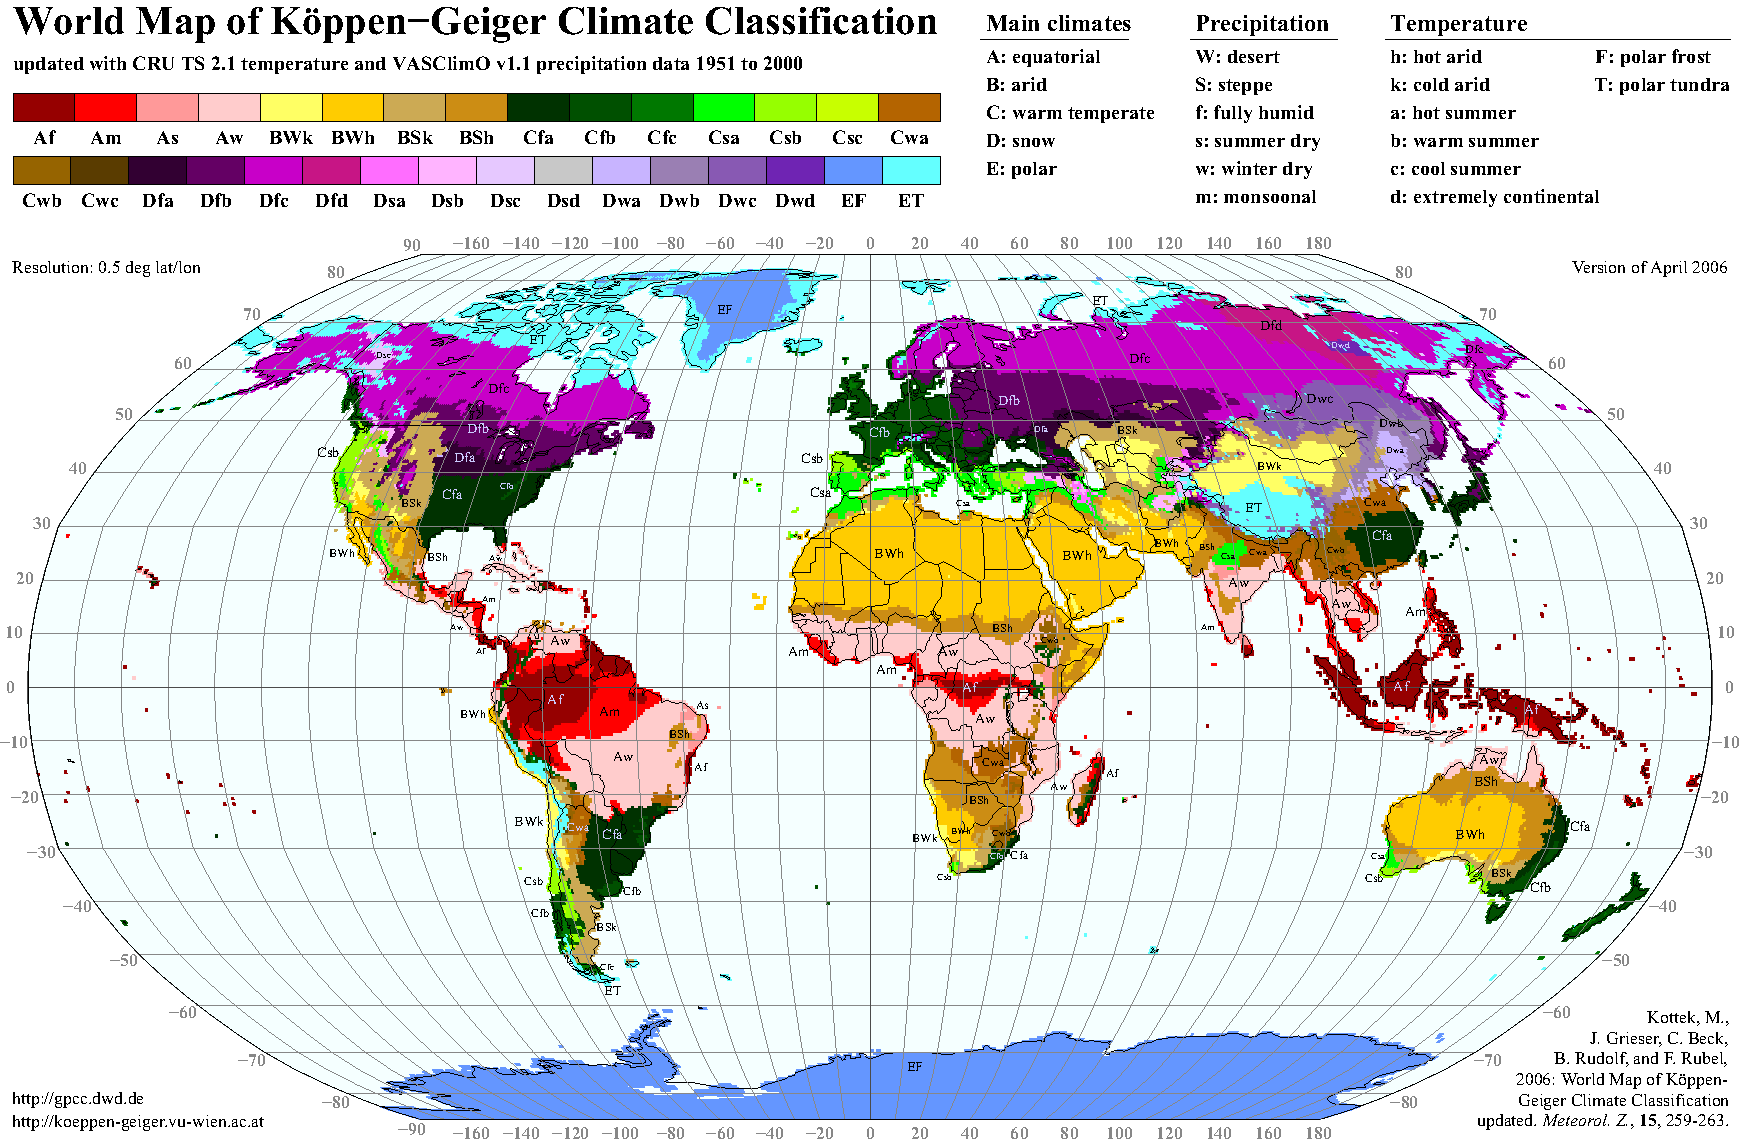
\includegraphics[width=0.95\linewidth]{figure/chapter1/kottek_et_al_2006_A4.pdf}
    \bicaption{全球Köppen-Geiger气候分区}{World Map of Köppen-Geiger Climate Classification}
    \label{fig:climate_zones}
\end{figure}

第二，数据层面，即现有数据产品难以同时兼顾全球覆盖、长期连续、中等空间分辨率和高时间分辨率等要求。统计分配型产品虽然实现了长时序全球覆盖，但空间和时间分辨率较粗，缺乏遥感识别意义上的稻田边界和像元级动态信息；遥感识别型产品虽然提升了空间细节，却往往局限于区域尺度或少数年份，难以提供长期、连续和像元级的动态生长季信息。对于稻田降温效应等依赖真实生长季窗口的研究而言，缺少逐日或像元级生长季信息会直接带来时间匹配误差和空间范围误判，使得环境效应评估的科学可信度受到根本制约。

第三，方法层面，即现有方法难以同时实现物候可解释性、时间序列适应性和全球稳定推广。物候规则法可解释性强但弹性不足，面对复杂复种制度和弱淹水信号时精度下降；机器学习方法局地精度高但泛化能力有限，对跨区域样本一致性和传感器稳定性要求苛刻；单纯时间序列匹配方法灵活性较好，但模板构建和阈值设置仍存在不确定性，难以处理全球范围内生长季长度的显著分异和多季种植信号的交错叠加。全球制图方法需要在普适性、可解释性和精度之间取得平衡，并形成能够长期稳定更新的数据生产框架。

因此，本研究需要发展一种能够适应全球复杂水稻种植制度的动态制图框架，并构建可支撑地表温度效应评估的全球水稻生长季数据产品。其核心目标不仅是回答"全球稻田在哪里"，还要进一步回答"全球稻田何时生长、持续多久、是否存在多季种植，以及这种变化如何影响地表气候"。这一数据与方法需求直接对应本研究第三章的方法构建和第四章的数据集开发，也为后续第五章的全球水稻时空格局分析、第六章和第七章的稻田地表降温效应评估提供了不可或缺的时空基础。

\section{稻田地表生物物理温度效应研究进展}

本节将稻田地表温度效应研究置于陆地表面生物物理效应的理论框架中进行系统综述，为后文第六章、第七章和第八章的研究设计奠定文献基础。首先界定地表温度（land surface temperature, LST）的概念、地表生物物理温度效应的作用机制及其与温室气体效应的本质区别，并阐明稻田生态系统的特殊性；其次从森林与自然植被、灌溉系统和农田管理三个维度梳理一般土地系统的地表温度效应研究进展，为理解稻田温度效应提供理论参照；随后按尺度由小到大系统梳理已有稻田温度效应研究；最后归纳该领域存在的主要不足，明确本文的研究空间。

\subsection{地表生物物理温度效应的概念与生物物理机制}

地表温度（land surface temperature, LST）是遥感热红外波段反演的地表辐射温度，反映地表皮肤层（skin layer）的能量平衡状态，其物理内涵与近地表空气温度（near-surface air temperature, $T_a$）存在本质差异。LST 直接受控于地表能量平衡方程中各分量的分配关系，对下垫面反照率、土壤湿度、植被覆盖度和蒸散发强度等参数高度敏感；而近地气温是大气边界层内的空气温度，受平流、湍流混合和大气辐射过程共同调制。因此，LST 的空间异质性通常强于气温，且两者在量级和响应时间上并非一一对应。在辐射强迫和大气环流背景相同的条件下，不同土地覆盖类型的 LST 差异可达数摄氏度，而近地气温由于湍流混合的均化作用，其差异往往明显小于 LST 差异\cite{Bright2017LCMC}。这一差异意味着，基于 LST 观测得到的地表温度效应，在向外推估近地气温响应时需要谨慎对待，不能直接等同。本文研究所称"冷岛效应"，在正文中限定为"稻田地表降温效应"或"稻田地表生物物理温度效应"，特指稻田在水稻生长季内相对于周边非稻田农田表现出的 LST 降低现象。本文研究的核心物理量是稻田相对于周边非稻田农田的 LST 差异（$\Delta$LST），而非直接估算全球平均近地气温的变化。这一界定意味着：本文揭示的稻田降温效应是地表能量平衡层面的生物物理响应，主要反映局地尺度的下垫面温度调节，不宜直接外推为全球或区域尺度气温变化的定量估计。选择"周边非稻田农田"作为比较基准，而非城市、林地或裸地，是为了将 LST 差异的归因聚焦于水稻种植本身的水分管理和冠层特性，而非跨土地覆盖类型的系统性差异。这一比较基准的选取策略，将在第六章的样本匹配设计中进一步展开论证。

土地覆盖类型和土地管理措施通过改变地表能量平衡的多个分量，进而影响 LST，其核心生物物理过程可从五个相互耦合的维度加以理解。第一，反照率（albedo）效应。地表反照率决定到达地表的太阳短波辐射有多少被反射回大气，反照率升高会减少地表净辐射吸收而倾向于降低地表温度，反之则增加辐射吸收而倾向于升温。不同土地覆盖类型的反照率差异显著：森林冠层因结构复杂通常具有较低反照率，而冰雪覆盖地表具有较高反照率；农田的反照率则随作物类型、生育阶段和土壤背景动态改变，直接影响生长季内的地表能量收支\cite{Duveiller2018Energy}。第二，蒸散发（evapotranspiration, ET）与潜热通量（latent heat flux, $\lambda E$）效应。蒸散发过程消耗能量用于水分相变，将本可转化为显热通量（sensible heat flux, $H$）的能量以潜热形式释放到大气中；在净辐射（$R_n$）相对稳定时，$\lambda E$ 的增加通常以 $H$ 的减少为代价，而 $H$ 是直接加热地表和近地表空气的主要途径，因此 ET 增强往往表现为 LST 降低。蒸散发包括土壤蒸发、植被冠层截留水分蒸发和植被蒸腾三个分量，其总和受土壤水分供给、植被覆盖度、叶面积指数（LAI）和大气蒸发需求共同控制\cite{Bright2017LCMC}。第三，土壤水分与热容量效应。土壤含水量的增加会提高地表热容量和热传导率，改变地表温度的日变化幅度和相位；湿润土壤的升温速率较慢，白天峰值温度较低，但夜间降温也相对缓慢。同时，充足的土壤水分供给是维持高 ET 的前提条件，因此土壤水分效应与蒸散发效应之间存在紧密的物理耦合。第四，冠层结构、地表粗糙度和显热/潜热分配效应。植被冠层通过改变地表粗糙度影响湍流交换效率，通过遮蔽土壤减少直接蒸发，并通过根系吸水维持蒸腾；不同植被类型和管理方式下，波文比（$H/\lambda E$）的差异直接决定了 LST 的方向和强度。高而密的冠层通常具有更大的粗糙度和更强的蒸腾能力，倾向于降低 LST；而稀疏或低矮植被则可能因土壤暴露增加而导致 LST 升高\cite{Chen2024Croplands}。第五，热储存效应。水体和湿润土壤具有较高的热容量，能够在白天储存更多热量并在夜间缓慢释放，使具有水层覆盖的下垫面表现出较小的日温度振幅，但其对白天和夜间平均温度的影响方向可能相反：白天储热倾向于降低升温幅度，夜间释热则倾向于减缓降温幅度。上述过程共同说明，地表生物物理温度效应是下垫面属性改变后通过能量平衡再分配产生的温度响应，其方向（降温或增温）和强度取决于多种竞争机制的综合结果。对于稻田而言，蒸散发增强和反照率变化的综合效应通常主导其 LST 特征，而水体热容量效应则调节其温度日变化节律。

地表生物物理温度效应与温室气体效应是土地覆盖和农业管理影响气候系统的两条独立路径，二者在作用过程、空间尺度和评价指标上均存在本质区别，不能进行简单叠加或等量抵消。温室气体效应主要对应大气辐射强迫（radiative forcing）和全球气候响应：稻田甲烷（CH$_4$）排放进入大气后，通过吸收和再发射长波辐射改变地球辐射收支，具有长期累积性、全球混合性和辐射强迫可量化特征，其气候影响通常以辐射强迫（W m$^{-2}$）或 CO$_2$ 当量度量，作用于全球尺度的大气成分变化，时间尺度可达数十年至数百年\cite{Qian2023RiceGHG,Zhang2020NatCommun}。在这一框架下，稻田作为甲烷排放源，其生物地球化学气候效应表现为增温贡献。地表生物物理温度效应则主要反映土地覆盖或土地管理改变下垫面属性后，通过反照率、蒸散发、热容量和粗糙度等过程改变局地或区域地表能量平衡，进而引起 LST 响应；其影响范围具有较强的局地性和季节性，依赖于具体下垫面状态和当时的大气强迫条件，通常以温度差值（$^{\circ}\mathrm{C}$）或能量通量变化（W m$^{-2}$）度量\cite{Bright2017LCMC,Duveiller2018Energy}。与温室气体效应不同，生物物理温度效应在大气中不留存，也不产生累积性辐射强迫，而是随土地覆盖状态的季节性变化而即时响应。因此，LST 降温效应与甲烷排放导致的温室气体增温效应属于不同过程、不同尺度和不同指标，不能直接等量抵消：前者是局地能量平衡的即时再分配，后者是全球辐射收支的累积扰动；前者以地表温度差异度量，后者以辐射强迫或 CO$_2$ 当量度量。本文研究稻田地表生物物理降温效应，目的在于补充现有对稻田气候效应的认识维度，而非对稻田总体气候净效应作出最终判断。只有在统一物理框架和统一量纲下完成综合权衡，才能科学回答稻田在气候系统上的综合效应问题。这一认识将在第八章综合讨论中进一步展开。

稻田生态系统地表温度效应的特殊性，根本上来自其不同于普通旱地农田的下垫面组成。一般旱地作物的地表能量分配主要受土壤水分供给、冠层覆盖度和作物蒸腾控制，而稻田在生长季内通常同时存在田面水、湿润土壤和水稻冠层，形成典型的水—植被复合下垫面。浅水层能够直接通过水面蒸发消耗可用能量，湿润土壤为蒸散过程提供持续水分供给，水稻冠层则在生长过程中逐步增强蒸腾作用和湍流交换。三者共同作用，使稻田能量平衡更倾向于将净辐射分配至潜热通量，而不是显热通量，从而具有降低白天地表温度的物理基础\cite{Xue2021RemoteSensing,Thiery2020Irrigation}。因此，稻田降温不能简单理解为由水层蒸发单独主导的现象，而应理解为水层蒸发、土壤湿度维持和冠层蒸腾共同改变显热/潜热分配的结果。

这种水层与冠层的耦合过程也使稻田区别于一般灌溉农田。灌溉小麦、玉米等旱地作物时，人为水分输入主要通过提高土壤湿度来解除蒸散发的水分限制；而稻田的水分管理并不是外加于旱地系统之上的辅助措施，而是水稻种植制度本身的组成部分。移栽、返青、分蘖、晒田、抽穗和成熟等阶段均伴随不同的水分管理目标，田面水层是否存在、水层深度、土壤饱和程度和冠层封闭度会同步改变。已有灌溉气候效应研究表明，人为水分输入能够显著影响地表温度和边界层过程\cite{McDermid2023Irrigation}；稻田则在这一机制基础上叠加了水稻作物特有的物候节律和阶段性淹水环境。因此，稻田温度效应既包含灌溉降温的一般机制，又具有水层—冠层—管理制度共同塑造的系统特殊性。

由于水分管理和冠层发育都随生育阶段变化，稻田地表温度效应还具有明显的时间依赖性。稻田并非全年维持同一种下垫面状态，也不应被视为具有固定降温强度的静态土地覆盖类型。在移栽或返青初期，田面浅水和裸露土壤比例较高，水面蒸发可能较强，但冠层尚未形成，植被蒸腾和遮阴作用有限；进入分蘖、拔节至抽穗阶段后，冠层覆盖度、叶面积指数和蒸腾强度逐步提高，潜热释放能力增强，地表温度响应可能随之加强；到成熟和收获阶段，冠层衰老、田间排水和残茬裸露会削弱蒸散发过程，使温度效应趋于减弱。由此可见，稻田温度效应是随生育阶段、水分管理和冠层结构共同演变的动态过程，而不是可以用年度平均土地覆盖类别直接代表的常量。

这种时间依赖性在昼夜尺度上同样明显。白天太阳辐射输入强，蒸发和蒸腾过程活跃，潜热通量增强更容易转化为可观测的 LST 降低；夜间短波辐射消失，蒸散发显著减弱，水体和湿润土壤的热容量、长波辐射释放以及近地层稳定度等过程相对重要，稻田与周边非稻田农田的温度差异可能明显缩小，甚至在特定条件下表现出不同方向。已有区域遥感研究已经提示，稻田温度效应具有昼夜不对称和生长季内变化特征\cite{Xue2021RemoteSensing,Liu2022AgForMet}。这一认识的意义在于，稻田降温效应不能脱离观测时段和生长阶段讨论；若使用固定月份或年度平均 LST 进行比较，就可能把移栽前、收获后、轮作期或错季种植信号混入分析，从而削弱温度差异的物理解释。后文第六章对稻田地表降温效应的量化方法，正需要以真实水稻生长季为时间约束；第七章对昼夜差异和生长季内过程的分析，也建立在这一理论判断之上。

稻田温度效应也嵌入具体的农田景观结构之中。与森林、草地等自然生态系统相比，稻田往往由田埂、沟渠、灌排系统和农户经营边界共同组织，其空间形态既受地形水文条件制约，也受农业工程和土地经营制度影响。田块规模、稻田比例和空间连续性会改变水分蒸散的空间集聚程度：破碎小斑块稻田更容易受到周边旱地、建设用地或裸地的边界影响，其 LST 响应可能被混合像元和邻近地表通量削弱；连片稻田则可能通过持续的高蒸散发、较高空气湿度和较一致的地表能量分配形成更稳定的局地冷却环境。因而，稻田地表温度效应不是单个像元的属性问题，而是与农田景观格局密切相关的空间过程。

这种空间过程的影响范围可能并不严格止于稻田边界。稻田与周边非稻田农田之间存在近距离的水汽交换、湍流混合和热量平流，尤其在连片稻田比例较高、地形开阔且背景风场有利的区域，稻田形成的较低地表温度可能影响邻近农田的热环境。这一潜在外溢效应对于理解农田景观格局、城郊热环境缓解和区域农业气候适应具有重要意义，但也增加了归因难度：若对照样本距离稻田过近，可能低估稻田与非稻田农田之间的真实温度差异；若距离过远，又可能引入地形、气候和土地管理差异。正因如此，稻田温度效应评估需要同时关注稻田比例、田块规模、空间邻近关系和对照样本匹配策略，而不能只报告一个区域平均 $\Delta$LST。

由此可见，稻田既不能被简单等同于普通旱地作物，也不能被完全归入一般灌溉农田；它是由水分管理、作物物候和农田景观格局共同塑造的特殊土地系统。认识稻田地表温度效应，需要在一般土地系统生物物理效应理论的基础上，进一步引入水稻真实生长季、昼夜差异、田块规模和邻近对照等约束。这样的理论铺垫为后续从一般土地系统研究进展转向稻田专门研究进展提供了逻辑衔接，也为第六章和第七章围绕生长季约束、样本匹配、昼夜对比与空间结构分析开展方法和结果设计奠定基础。

\subsection{地表生物物理温度效应的研究进展}

本节将稻田地表温度效应研究置于更宏观的土地系统科学背景中加以定位，随后聚焦稻田本身的温度效应研究进展。

\subsubsection{一般土地系统的地表温度效应研究进展}

森林和自然植被覆盖变化的地表温度效应研究是土地系统生物物理气候效应领域中发展较为成熟的板块。已有研究从局地观测、区域遥感和全球模型模拟等多个尺度证实，森林覆盖变化能够通过蒸散发和反照率的竞争过程显著影响 LST\cite{Alkama2016}。森林研究的理论价值在于：它确立了土地覆盖变化$\rightarrow$能量平衡再分配$\rightarrow$LST 响应这一分析框架，并揭示了温度效应的方向和强度受纬度、季节、水分条件和反照率变化共同控制的基本规律。例如，Li 等基于全球遥感观测的研究指出，森林的冷却或增温效应取决于蒸散发增强与反照率降低之间的竞争关系，热带森林通常因强蒸散发而表现出显著的冷却效应，而高纬度森林因反照率降低可能表现出不同的温度效应方向甚至冬季增温信号\cite{Li2015NatCommun}；Alkama 和 Cescatti 在 \textit{Science} 发表的研究进一步从全球森林覆盖变化角度说明，土地覆盖变化通过生物物理过程对局地气候的影响具有明确的纬度和季节分异规律\cite{Alkama2016}。这些发现为后续农田和灌溉系统的温度效应研究提供了可参照的生物物理机制和分析范式\cite{Bright2017LCMC}。然而，森林与稻田在下垫面属性上存在本质差异。森林为多年生深根系植被，全年维持较高叶面积指数和蒸腾能力，其温度效应具有较强的全年持续性和空间稳定性；稻田则为一年生作物，其水层状态、冠层发育和蒸散强度在年内呈显著阶段性变化，温度效应仅在生长季内表现突出，收获后或休耕期则大幅减弱甚至消失。此外，森林冠层结构复杂、地表粗糙度高，能量分配过程与水稻冠层存在显著差异。因此，森林温度效应研究主要提供机制层面的参照框架，不能直接套用于理解稻田的温度效应规律。将稻田温度效应研究纳入土地系统科学视野时，需要充分认识到一年生作物系统的季节性和人为管理依赖性所带来的独特性。

灌溉农田的地表温度效应研究与稻田具有高度相似性，因为二者均涉及人为水分输入、土壤水分增加和潜热通量增强。Thiery 等结合观测和模型证据指出，灌溉扩张能够通过增强蒸散发显著缓解局地极端高温，在南亚等灌溉农业区效应尤为明显\cite{Thiery2020Irrigation}。灌溉降温的物理机制在于：人为水分输入打破了自然水分供给对蒸散发的限制，使土壤蒸发和作物蒸腾得以在干燥气候条件下维持较高水平，从而将更多可用能量分配至潜热通量，减少显热通量和地表升温。McDermid 等进一步从全球尺度评估了灌溉的气候效应，指出灌溉不仅改变地表温度，还通过水汽反馈影响边界层结构和降水过程\cite{McDermid2023Irrigation}。这些灌溉降温研究为理解稻田温度效应提供了直接参照：如果一般性的灌溉农田即可通过水分输入改变局地热环境，那么具有长期或阶段性淹水、且同时伴随作物蒸腾的稻田，理论上应具有更强或更特殊的温度调节效应。灌溉研究与稻田研究的关键差异在于：灌溉农田的水分管理通常以土壤湿度提升为主，作物蒸腾是潜热释放的主要来源，而稻田具有可见水层覆盖和特有的水稻冠层发育过程，水面蒸发在生长季初期甚至整个生育期均可能贡献显著的潜热通量；此外，灌溉研究的关注对象多为小麦、玉米等旱地作物在灌溉条件下的温度响应，而稻田是天然的水—植被复合系统，其水分条件并非对旱地作物的补充，而是系统固有的下垫面属性。因此，稻田既具备灌溉系统的水分管理特征，又叠加了水稻作物的生物学特性和淹水环境的水文特性，其温度效应不能简单等同于一般灌溉降温，而应在灌溉研究的基础上进一步考察水层—冠层—人为管理三者耦合的独特机制。

农田管理措施的地表温度效应研究表明，同类耕地上的温度响应不仅取决于作物类型，还受灌溉方式、作物历、耕作制度、覆盖度和土壤水分状况的显著影响\cite{Chen2024Croplands}。不同作物因冠层结构、根系深度和蒸腾系数的差异，在相同气候背景下可能表现出不同的 LST 特征：例如，大豆和玉米的蒸腾系数差异导致其在生长旺盛期具有不同的能量分配格局。同一作物在不同灌溉制度、播栽期和种植密度下，其能量平衡分配也存在明显分异。保护性耕作、覆盖作物和秸秆还田等措施通过改变土壤水分保持能力和地表覆盖度，进一步调节农田的蒸散发过程和温度响应。这些研究表明，农田地表温度效应是土地覆盖类型、作物属性、水分管理和人为制度多因素耦合的结果，不能简化为单一作物类型或土地覆盖标签的温度属性。上述研究共同说明：农田地表温度效应是土地覆盖类型、作物属性、水分管理和人为制度多因素耦合的结果。稻田作为水分管理、作物生长和人为制度高度耦合的典型农田系统，其地表温度效应既属于土地覆盖生物物理效应研究的一部分，也具有区别于森林、旱地农田和一般灌溉系统的特殊性。理解稻田温度效应，需要在一般土地系统生物物理效应的理论框架下，充分考虑稻田特有的水层动态、作物物候节律和人为管理变异性。这一认识为后文从"一般土地系统"聚焦到"稻田专门系统"提供了自然的理论过渡。

\subsubsection{稻田生态系统的地表温度效应研究进展}

早期稻田温度效应研究多集中于局地尺度，关注稻田对夏季近地气温、城市边缘热环境或局地小气候的调节作用。例如，Yokohari 等基于东京住宅区周边气象观测的研究较早认识到，保留稻田湿地能够在夏季高温期产生一定的局地冷却功能，对缓解城市热岛具有潜在价值\cite{Yokohari2001}。这类研究通常采用定点气象站或移动观测手段，在稻田与周边建筑用地、裸地或旱地之间进行温度对比，其主要贡献在于首次从观测角度证实了稻田具备不同于周边建设用地的温度调节能力，将稻田从单纯的粮食生产单元重新定位为具有气候调节功能的土地系统类型。然而，局地观测研究的局限也十分明显：气象站点数量有限、空间覆盖范围小、持续时间通常较短，且多为近地气温而非地表辐射温度的观测。这些研究能够说明"稻田在特定地点可能降温"的现象存在，但难以回答稻田降温是否具有区域或全球普遍性，也无法比较不同气候区、不同种植制度和不同田块形态下的效应差异。此外，局地观测往往缺乏严格的对照实验设计，温度差异容易受到地形、微气候和观测高度等混淆因素影响。因此，尽管局地观测研究奠定了稻田温度效应的早期认识基础，但要将这一认识从"局地现象"提升为"一般规律"，需要借助空间连续观测手段和更大尺度的分析框架。

近年来，卫星遥感 LST 数据的发展使稻田温度效应研究从稀疏的局地观测扩展到连续的区域尺度。遥感手段能够在统一物理基准上获取大范围、重复观测的地表温度信息，为比较稻田与非稻田农田的 LST 差异提供了可能。已有研究在东北亚、韩国、日本以及中国部分稻区开展了基于遥感 LST 的稻田温度效应评估\cite{Xue2021RemoteSensing}。这些研究普遍表明，稻田在生长季白天相较周边土地覆盖类型具有更低的 LST，且降温效应表现出明显的昼夜不对称性和生长季内动态变化特征。例如，Liu 等基于 MODIS LST 在东北亚地区的分析发现，稻田白天 LST 显著低于周边旱地，而夜间差异大幅缩小\cite{Liu2022AgForMet}，且降温效应随生育阶段呈动态变化。这些区域遥感研究的价值在于：证实了稻田降温并非个别站点的局地现象，而是在具有一定空间连续性的稻区内普遍存在的生物物理响应；同时，遥感数据也使得降温效应与蒸散发、土壤水分和植被指数之间的定量关系得以建立。然而，现有区域研究通常局限于单一国家或若干相邻行政区域，其对照样本构建方法、生长季定义方式和空间匹配策略也不尽相同，研究结果之间的可比性受到一定限制。例如，部分研究将稻田与林地或裸地比较，其温度差异主要反映土地覆盖类型效应，难以将降温归因于水稻种植本身；部分研究采用固定月份定义生长季，未充分考虑区域内水稻播栽期的空间差异。此外，区域研究仍难以覆盖全球主要水稻种植区，尤其缺乏对非洲、美洲和南亚大范围稻区的系统分析。因此，区域遥感研究虽然显著推进了对稻田温度效应的空间认识，但其结论的外推性和全球代表性仍然有限。

目前，全球尺度稻田地表温度效应的系统评估仍然较为稀缺。这一缺失不仅源于全球连续 LST 遥感数据的可获取性和处理复杂性，更根本的限制在于缺乏能够提供全球一致、长期连续、真实生长季和较高空间分辨率的稻田动态数据产品，以及对照样本构建方法的不统一。全球稻田温度效应评估要求同时满足以下数据条件：第一，全球覆盖且空间分辨率足以刻画稻田斑块与周边农田空间关系的稻田分布数据，以支持田块规模和空间邻近效应分析；第二，能够反映真实水稻生长季起止时间的动态信息，以避免固定月份造成的时序错配，尤其在热带多熟区和跨纬度稻区；第三，长期连续的时间覆盖，以支撑多年平均效应估计和年际变化分析，降低单一年份气候异常带来的不确定性；第四，统一构建的周边非稻田农田对照样本，以控制土地覆盖类型以外的混淆因素，增强归因可信度。现有数据产品往往只能满足上述条件的一部分：粗分辨率统计分配型产品缺乏精细空间结构和生长季动态；高分辨率区域水稻图难以支撑全球一致分析；年度静态土地覆盖图无法识别水稻真实生育期。因此，全球稻田地表温度效应研究面临的瓶颈，本质上是一个数据基础问题。这恰恰说明：构建兼具全球覆盖、中等空间分辨率、长期连续和日尺度生长季信息的水稻动态数据集，不仅是制图学科的任务，也是开展全球稻田生物物理气候效应评估不可或缺的数据前提。值得强调的是，本节关注的是稻田温度效应研究本身的尺度进展与不足，而非水稻制图产品和方法的不足，后者已在 1.2 节中系统论述。

\subsection{稻田生态系统地表温度效应研究的主要不足}

基于上述文献综述，本节围绕稻田地表温度效应研究存在的问题意识，归纳五个主要不足。每一项不足均说明：已有研究为何存在局限，该局限为何重要，以及本文后续章节如何回应。

现有稻田降温研究多集中在局地、国家或区域尺度，例如日本、韩国、东北亚和中国部分省份的实证分析。这些研究能够证明降温现象在特定区域存在，但难以判断稻田降温是否在全球主要水稻种植区普遍发生，也难以比较不同气候区、不同田块形态、灌溉制度和复种制度下的效应差异。非洲稻区、美洲稻区和南亚大范围稻区的温度效应几乎处于研究空白状态，而这些区域在气候背景、水分条件、田块规模和管理方式上与东北亚和东亚稻区存在显著差异。全球普遍性的缺失，使稻田降温效应始终停留在"区域现象"层面，无法上升为全球土地系统科学问题，也限制了将区域经验向全球尺度外推的可信度。此外，不同气候区的水分条件和蒸散发潜力差异，可能导致降温效应的方向和强度呈现系统性区域分异；若缺乏全球覆盖的分析，这些区域调控规律将难以被识别和比较。本文后续第七章将基于 GlobalRice500 数据集，在全球主要稻区系统评估稻田白天和夜间 LST 差异的空间格局，揭示各大洲、各气候区的降温差异与调控规律，从而将稻田降温效应从区域经验提升为全球土地系统问题的系统证据。

许多研究采用固定月份、固定季节或基于气候区平均作物历来定义水稻生长阶段，但全球水稻播栽期、生长季长度和复种制度差异显著。在温带单季稻区，固定月份（如北半球 6 至 9 月）可能基本覆盖水稻生育期；但在亚热带双季稻区，固定窗口可能仅覆盖单季而遗漏另一季，或将两季之间的休耕期错误纳入；在热带多熟区，水稻生长月份并不固定，全年均可能存在活跃生长季，固定时间窗极易混入非生长季、休耕期或错季阶段。生长季过程刻画不足的直接后果是：观测到的温度差异难以准确归因于水稻生长和稻田蒸散过程，而非生长季或轮作作物的温度信号会系统性地稀释或扭曲降温效应估计。尤其对于年内多季种植区域，若无法精确识别每一季的起止时间，LST 差异将沦为混合了多季、休耕和非水稻期的模糊信号，失去物理可解释性。本文后续第六章将基于 GlobalRice500 提供的逐像元 SOS--EOS 信息，严格约束真实水稻生长季窗口，实现像元级动态时间匹配，从而将 LST 分析的时间基准从"固定月份"提升至"真实生育期"，显著增强温度差异归因的精确性。

稻田与非稻田的温度差异可能受到地形、气候背景、土地覆盖、土壤水分、灌溉条件和空间邻近关系的影响。若将稻田直接与城市、林地或裸地比较，LST 差异主要反映土地覆盖类型效应，难以将温度差异归因于稻田本身；即便与农田比较，若缺乏海拔、距离和背景条件的约束，仍可能引入地形和微气候偏差。例如，低海拔河谷稻田与高海拔山坡旱地之间的温度差异，可能主要由海拔梯度而非水稻种植导致；远离水体源区的旱地与邻近灌溉渠的稻田之间的差异，可能反映的是灌溉可及性而非作物类型效应。对照样本构建方法不统一，是现有研究结论可比性差的重要原因：不同研究采用不同的比较基准和空间筛选策略，使得其结果之间难以进行横向对比和元分析。归因控制的不足，还导致现有研究无法可靠区分"稻田效应"与"水分管理效应""地形效应""景观背景效应"的贡献份额。本文第六章将通过非稻田农田样本匹配、同一 10 km 网格约束、海拔约束和背景条件控制，增强稻田降温效应归因的可信度。通过将比较基准严格限定为空间邻近、环境相似的非稻田农田，并控制地形和宏观气候背景，本文力求将观测到的 LST 差异最大限度地归因于水稻种植本身的水分管理和冠层特性。

现有研究多关注稻田平均降温强度，对稻田比例、田块规模、空间连续性以及稻田降温是否影响周边非稻田区域关注不足。然而，如果降温效应随稻田景观格局显著变化，那么单纯报告全球或区域平均 $\Delta$LST 将掩盖重要的空间异质性信息；如果降温存在空间外溢，则稻田气候效应评估不应局限于稻田本身，而应考虑其对周边农田小气候的区域性影响。景观结构认识的缺失，限制了将遥感观测结果向农业景观规划和区域气候管理转化的能力。例如，在城郊热环境调控和农田景观优化中，了解稻田比例阈值、斑块规模效应和外溢距离是制定空间策略的前提；若缺乏这些知识，政策制定者无法判断保留多大面积的连片稻田才能产生可感知的局地气候调节效果。此外，景观结构还可能与降温效应之间存在非线性关系：小规模破碎化斑块可能因边界效应主导而降温微弱，而大规模连片稻田则可能通过区域湿度场协同产生放大效应，这种非线性在现有研究中尚未得到充分刻画。本文第七章将通过稻田比例梯度分析、斑块规模分级比较和非稻田梯度环带（NGR）设计，系统回应景观结构与外溢效应问题，揭示稻田空间格局对降温效应的调控规律及其对周边农田的热环境影响范围。

LST 降温效应可以补充稻田气候效应研究，但已有研究对其与温室气体增温效应、水资源消耗、产量收益和区域气候反馈之间的边界与关系讨论不足。部分表述存在将 LST 降温直接与甲烷增温抵消的逻辑风险，这在科学上是不严谨的。LST 降温效应与温室气体增温效应属于不同过程、不同尺度和不同指标，不能直接等量抵消；此外，LST 不等同于近地气温，局地地表降温也不等同于区域或全球气温响应。如果不对这些边界加以明确，稻田生物物理效应研究就可能被误读为对稻田总体气候净效应的最终判断，从而引发"稻田降温可以弥补甲烷排放"的过度推断。更为复杂的是，稻田降温效应以蒸散发增强为代价，这意味着其背后存在水资源消耗；若将降温视为气候收益而忽略水资源的区域约束，则同样是一种片面的认识。因此，厘清 LST 降温效应在稻田综合气候效应评估中的定位、边界和局限，是确保研究结论科学严谨性的必要环节。本文第八章将专门讨论 LST 降温、温室气体排放、水资源消耗和产量收益之间的边界与关系，明确本文研究在稻田综合气候效应评估中的定位与局限，避免将局地生物物理效应过度外推为全球气候收益。

综上，现有稻田地表温度效应研究在尺度覆盖、时间过程、归因控制、景观结构和效应边界五个维度上均存在明显不足。这些不足既制约了对稻田生物物理气候效应的完整认识，也直接指向了本文在方法构建、数据集开发和全球效应评估方面的研究空间。在此背景下，下一节将综合 1.1、1.2 和 1.3 的文献分析，凝练当前研究的核心不足与关键科学问题。

\section{研究内容与技术路线}

\subsection{科学问题}

前述研究背景与文献综述表明，全球稻田遥感监测及其地表生物物理降温效应研究并不是两个彼此孤立的议题。水稻制图为气候效应评估提供空间和时间边界，地表温度效应研究则反过来要求水稻数据不仅能够给出年度稻田范围，还要能够刻画真实生长季、长期变化和稻田空间结构。现有研究已经在区域水稻制图、统计型水稻数据集、灌溉降温和局地稻田小气候效应等方面积累了重要基础，但仍缺乏一条从全球稻田识别、数据产品构建、时空格局分析到稻田地表温度效应评估的完整证据链。因此，本文的科学问题不只是提高某一类分类精度，也不只是报告某一区域的 LST 差异，而是要回答全球水稻这一特殊水—植被—人为管理复合农田系统如何被稳定识别、如何随时间变化，以及这种变化如何影响地表热环境。

第一类科学问题是全球稻田动态数据缺口问题。已有全球作物或水稻数据产品在全球覆盖、长期连续、空间分辨率和生长季信息之间往往只能满足部分条件。统计分配型产品能够提供宏观面积信息，却难以反映像元尺度稻田边界和真实生长季过程；区域遥感产品空间分辨率较高，但覆盖范围和时间一致性不足；已有全球水稻产品虽然可用于面积统计，却通常缺少日尺度 SOS、EOS、生长季长度和复种制度等动态信息。对于 2001--2022 年全球水稻时空变化分析而言，缺乏稳定可靠、全球一致、日尺度、500 m 分辨率的水稻动态数据集，将直接限制对全球稻田扩张、收缩、区域转移和生长季差异的认识。对于稻田降温效应评估而言，这一数据缺口还会进一步造成 LST 时间窗口错配，使温度差异难以准确归因于水稻生长和稻田水分管理过程。

第二类科学问题是全球复杂种植制度下的水稻遥感识别方法问题。全球稻田并不是固定月份内出现的单一作物类型，而是受气候背景、灌溉条件、播栽制度、复种制度、品种熟期和农户管理共同控制的动态农田系统。温带单季稻区、亚热带双季稻区、热带多熟稻区、雨养低地稻区和机械化灌溉稻区在水分信号、植被指数曲线、生长季长度和年内周期数量上均存在显著差异。固定阈值和固定物候窗口方法具有可解释性，但难以适应播栽期高度不确定和多季种植并存的全球稻区；监督机器学习和深度学习方法在样本充足区域可以获得较高精度，但跨区域、跨年份和跨管理制度的泛化能力仍受训练样本一致性和长期更新稳定性制约；单纯时间序列匹配方法能够容忍一定物候相位差异，却仍需解决候选生长季搜索、曲线长度差异和多季稻连续识别问题。因此，本文需要回答的核心方法问题是：如何在全球复杂气候区和多样种植制度下，稳定识别不同播栽期、生长周期和复种制度的稻田，并使方法同时具备物候可解释性、时序弹性和长期可迁移性。

第三类科学问题是基于真实水稻生长季的稻田地表生物物理降温效应问题。已有稻田温度效应研究多证明局地或区域尺度稻田具有降温现象，但全球尺度上稻田相对于周边非稻田农田究竟具有多强的 LST 降低效应、这种效应在白天和夜间是否一致、在水稻生长季内如何随水层和冠层变化而演化、又如何受稻田比例、田块规模和空间邻近关系调控，仍缺乏系统认识。尤其是在全球水稻生长季高度异质的背景下，若采用固定月份或区域平均作物历进行温度比较，就可能将非生长季、轮作期或错季水稻混入分析，从而削弱物理解释。因此，本文需要在真实 SOS--EOS 约束下构建稻田与邻近非稻田农田的对照框架，量化全球稻田地表降温效应的强度、昼夜差异、生长季过程和空间结构调控机制，并明确这一 LST 降温效应与甲烷排放、水资源消耗和近地气温响应之间的边界。

上述三个科学问题具有递进关系。数据问题回答“全球稻田在哪里、何时生长以及如何变化”，方法问题回答“如何在全球复杂稻作制度下获得可信的水稻动态信息”，效应问题回答“在真实水稻生长季基础上，稻田如何影响地表温度以及这种影响意味着什么”。围绕这一逻辑，本文形成“全球稻田为何难以识别--如何构建普适制图方法--如何形成可信数据产品--全球水稻格局如何变化--稻田如何影响地表温度--这种影响的机制、意义与局限是什么”的研究主线。

\subsection{研究目标}

本文以全球水稻种植区为研究对象，综合利用长时间序列 MODIS 遥感数据、耕地与土地覆盖数据、已有高分辨率水稻参考图、国家统计数据、地表温度数据和地形数据，发展适用于全球复杂水稻种植制度的日尺度水稻动态遥感识别方法，构建 2001--2022 年全球 500 m 分辨率、日尺度水稻动态数据集 GlobalRice500，并基于该数据集揭示全球水稻时空变化格局，进一步量化 2003--2020 年全球稻田在真实生长季内的地表生物物理降温效应及其昼夜差异、生长季过程、田块规模效应和空间外溢特征。本文的总体目标是形成从方法构建、数据产品、格局揭示到气候效应评估的完整研究体系，为全球农业遥感、土地系统科学和农业气候效应研究提供数据基础和科学证据。

围绕这一总体目标，本文设置四个相互衔接的具体目标。首先，构建全球适用的水稻动态遥感识别方法。针对全球水稻播栽期不固定、生长季长度差异大、单季稻与多季稻并存、固定物候窗口难以适用等问题，融合水稻淹水--返青--生长--收获过程的物候先验知识与时间序列曲线匹配思想，建立 Moving Phenological Detection 与 Dynamic Time Warping 相结合的 MPD\_DTW 框架，实现逐像元、逐日尺度的水稻生长季识别。

其次，构建并验证全球长期水稻动态数据集 GlobalRice500。基于 2000--2023 年 MODIS 长时间序列遥感数据，生成 2001--2022 年全球 500 m 分辨率、日尺度水稻动态数据集，系统评估其空间识别精度、国家尺度面积一致性和主要不确定性来源，并从空间分辨率、时间范围、时间分辨率、全球覆盖能力和生长季信息等维度与已有水稻数据产品进行比较，明确其作为全球水稻环境效应评估数据基座的可靠性和适用边界。

再次，揭示 2001--2022 年全球水稻时空动态格局。利用 GlobalRice500 分析全球水稻面积年际变化、长期趋势、洲际差异、国家贡献、扩张与收缩热点以及典型区域变化过程，并进一步刻画 SOS、EOS、生长季长度、单季稻、双季稻和多季稻的空间分异，使全球水稻研究从静态面积统计扩展到生长季过程和复种制度动态监测。

最后，量化全球稻田地表生物物理降温效应及其空间调控机制。基于 GlobalRice500 提供的真实水稻生长季信息，构建稻田与邻近非稻田农田的 LST 对照框架，分别计算昼间和夜间 $\Delta$LST，揭示全球稻田生长季地表降温效应的空间分布、生长季内变化过程和昼夜不对称性，并分析稻田比例、田块规模和周边非稻田梯度环带对降温效应的调控作用。在此基础上，进一步讨论稻田降温效应的生物物理机制、科学意义与局限，明确其与温室气体增温效应之间不能直接等量抵消的边界。

\subsection{研究内容}

围绕上述科学问题和研究目标，本文首先开展全球水稻动态识别的数据基础与对象差异分析。水稻遥感制图的难点来自水—植被复合下垫面、人为水分管理和全球稻作制度差异，因此本文在数据源与预处理章节中系统梳理全球主要水稻种植区的物候差异和管理特征，构建用于水稻动态识别与 LST 效应评估的统一数据体系。该部分包括 MODIS 反射率及植被指数数据、耕地和土地覆盖数据、高分辨率水稻参考图、国家统计数据、LST 数据和 DEM 数据的获取、质量控制、时间序列重建、空间重采样和格式统一。其核心任务不是简单罗列数据源，而是说明为什么全球水稻制图必须依赖高时间分辨率时间序列、为什么真实 SOS--EOS 对后续温度效应评估不可替代，以及各类辅助数据如何共同约束非耕地、水体、地形和对照样本误差。

在方法构建方面，本文建立 MPD\_DTW 全球水稻动态识别框架。MPD 模块依据水稻移栽或返青初期的淹水信号搜索候选 SOS，并结合成熟收获后植被指数下降特征确定候选 EOS；DTW 模块比较候选生长季内像元 NDVI 曲线与标准水稻曲线之间的形态相似性，从而判断该候选生长季是否属于水稻生长季。二者之间的反馈机制是方法的关键：若当前 SOS--EOS 曲线被判定为水稻，则下一轮搜索从当前 EOS 之后开始，以避免不同生长季之间的时间重叠；若未被判定为水稻，则从当前 SOS 之后继续移动搜索，从而适应单季稻、双季稻和多季稻并存的全球稻作制度。在此基础上，本文进一步分析洪水因子、生长季长度约束和 DTW 距离阈值等关键参数的确定依据，并通过敏感性分析和适用性讨论评估该方法在热带多熟区、温带单季稻区、弱淹水信号区、旱直播稻区和田块破碎区的可靠性与局限。

在数据产品构建与全球水稻格局分析方面，本文基于 MPD\_DTW 方法生成 GlobalRice500，并从空间验证、统计验证、产品比较和不确定性分析四个方面评估数据产品可信度。空间验证利用不同洲和典型稻区的高分辨率水稻图或政府作物图评价像元尺度识别精度；统计验证将遥感面积与 FAO 等国家尺度统计数据进行比较，检验长期面积一致性；产品比较从全球覆盖、时间范围、空间分辨率、时间分辨率和生长季信息等维度说明 GlobalRice500 的独特贡献；不确定性分析重点讨论混合像元、稻田破碎化、弱淹水信号、验证数据分布不均和统计口径差异等问题。在数据可靠性评价基础上，本文进一步分析 2001--2022 年全球水稻面积变化、生长季特征、复种制度格局、洲际差异、国家差异和典型区域变化过程，从而使 GlobalRice500 不仅作为制图产品存在，也作为揭示全球水稻土地系统变化的科学数据基础。

在稻田地表降温效应评估方面，本文以真实水稻生长季内邻近非稻田农田 LST 与稻田 LST 之差定义 $\Delta$LST，并以 $\Delta$LST 为正表示稻田相对周边非稻田农田更冷。为增强归因可信度，非稻田对照样本限定为周边农田，而不与城市、林地、裸地或水体直接比较，并结合空间邻近、海拔、样本数量和背景条件约束降低地形和土地覆盖差异带来的偏差。基于该方法，本文分别计算昼间和夜间 $\Delta$LST，分析全球稻田降温效应空间格局、生长季内变化过程和昼夜差异；进一步通过 10 km 网格内稻田比例、稻田斑块规模和非稻田梯度环带 NPL 等指标，评估稻田景观结构对降温强度及外溢范围的影响。最后，本文在综合讨论中从能量平衡、潜热通量增强、显热通量减少、水层和冠层共同作用等角度解释稻田降温机制，并讨论 GlobalRice500 与稻田降温效应研究在农业遥感、土地系统科学、区域热环境调节和农业气候适应中的意义与局限。

\subsection{技术路线}

本文技术路线按照“科学问题提出--算法框架开发--数据底座构建--全球时空格局分析--地表降温效应量化--机制解释与综合讨论”的逻辑展开。第一章在全球水稻遥感制图研究和稻田地表生物物理温度效应研究综述的基础上，凝练数据、方法和效应三个层面的科学问题。第二章构建覆盖水稻动态识别和稻田降温效应评估的数据体系，重点说明全球稻作制度差异、MODIS 植被指数时间序列、辅助土地覆盖数据、LST 数据和 DEM 数据的预处理流程。第三章围绕全球水稻制图方法创新，建立 MPD\_DTW 框架，阐明 MPD 模块、DTW 模块、二者反馈机制以及参数设置与敏感性分析。

第四章和第五章构成 GlobalRice500 数据产品及其科学应用部分。第四章基于 MPD\_DTW 构建全球长期水稻动态数据集，并通过高分辨率参考图、国家统计数据、已有产品对比和不确定性分析评估其可信度；第五章进一步利用 GlobalRice500 揭示 2001--2022 年全球水稻面积变化、洲际和国家尺度格局、生长季特征、复种制度以及典型区域动态。通过这一安排，本文先回答数据产品是否可靠，再回答全球水稻时空格局如何变化，避免将未经验证的数据直接用于科学解释。

第六章和第七章构成稻田地表降温效应的方法与结果部分。第六章定义 $\Delta$LST 指标，建立稻田与邻近非稻田农田样本匹配方法，并说明真实水稻生长季约束、昼夜差异分析、稻田比例、田块规模和外溢效应量化方法；第七章在该方法基础上评估全球稻田昼间和夜间地表降温格局、生长季内过程、稻田比例效应、田块规模效应和周边非稻田区域外溢效应。第八章从 MPD\_DTW 框架理论意义、GlobalRice500 数据贡献、稻田降温机制、气候效应边界和研究局限等方面进行综合讨论；第九章总结主要结论、创新点与未来展望。本论文的总体研究框架见图\ref{fig:framework}。

\begin{figure}[htbp]
    \centering
    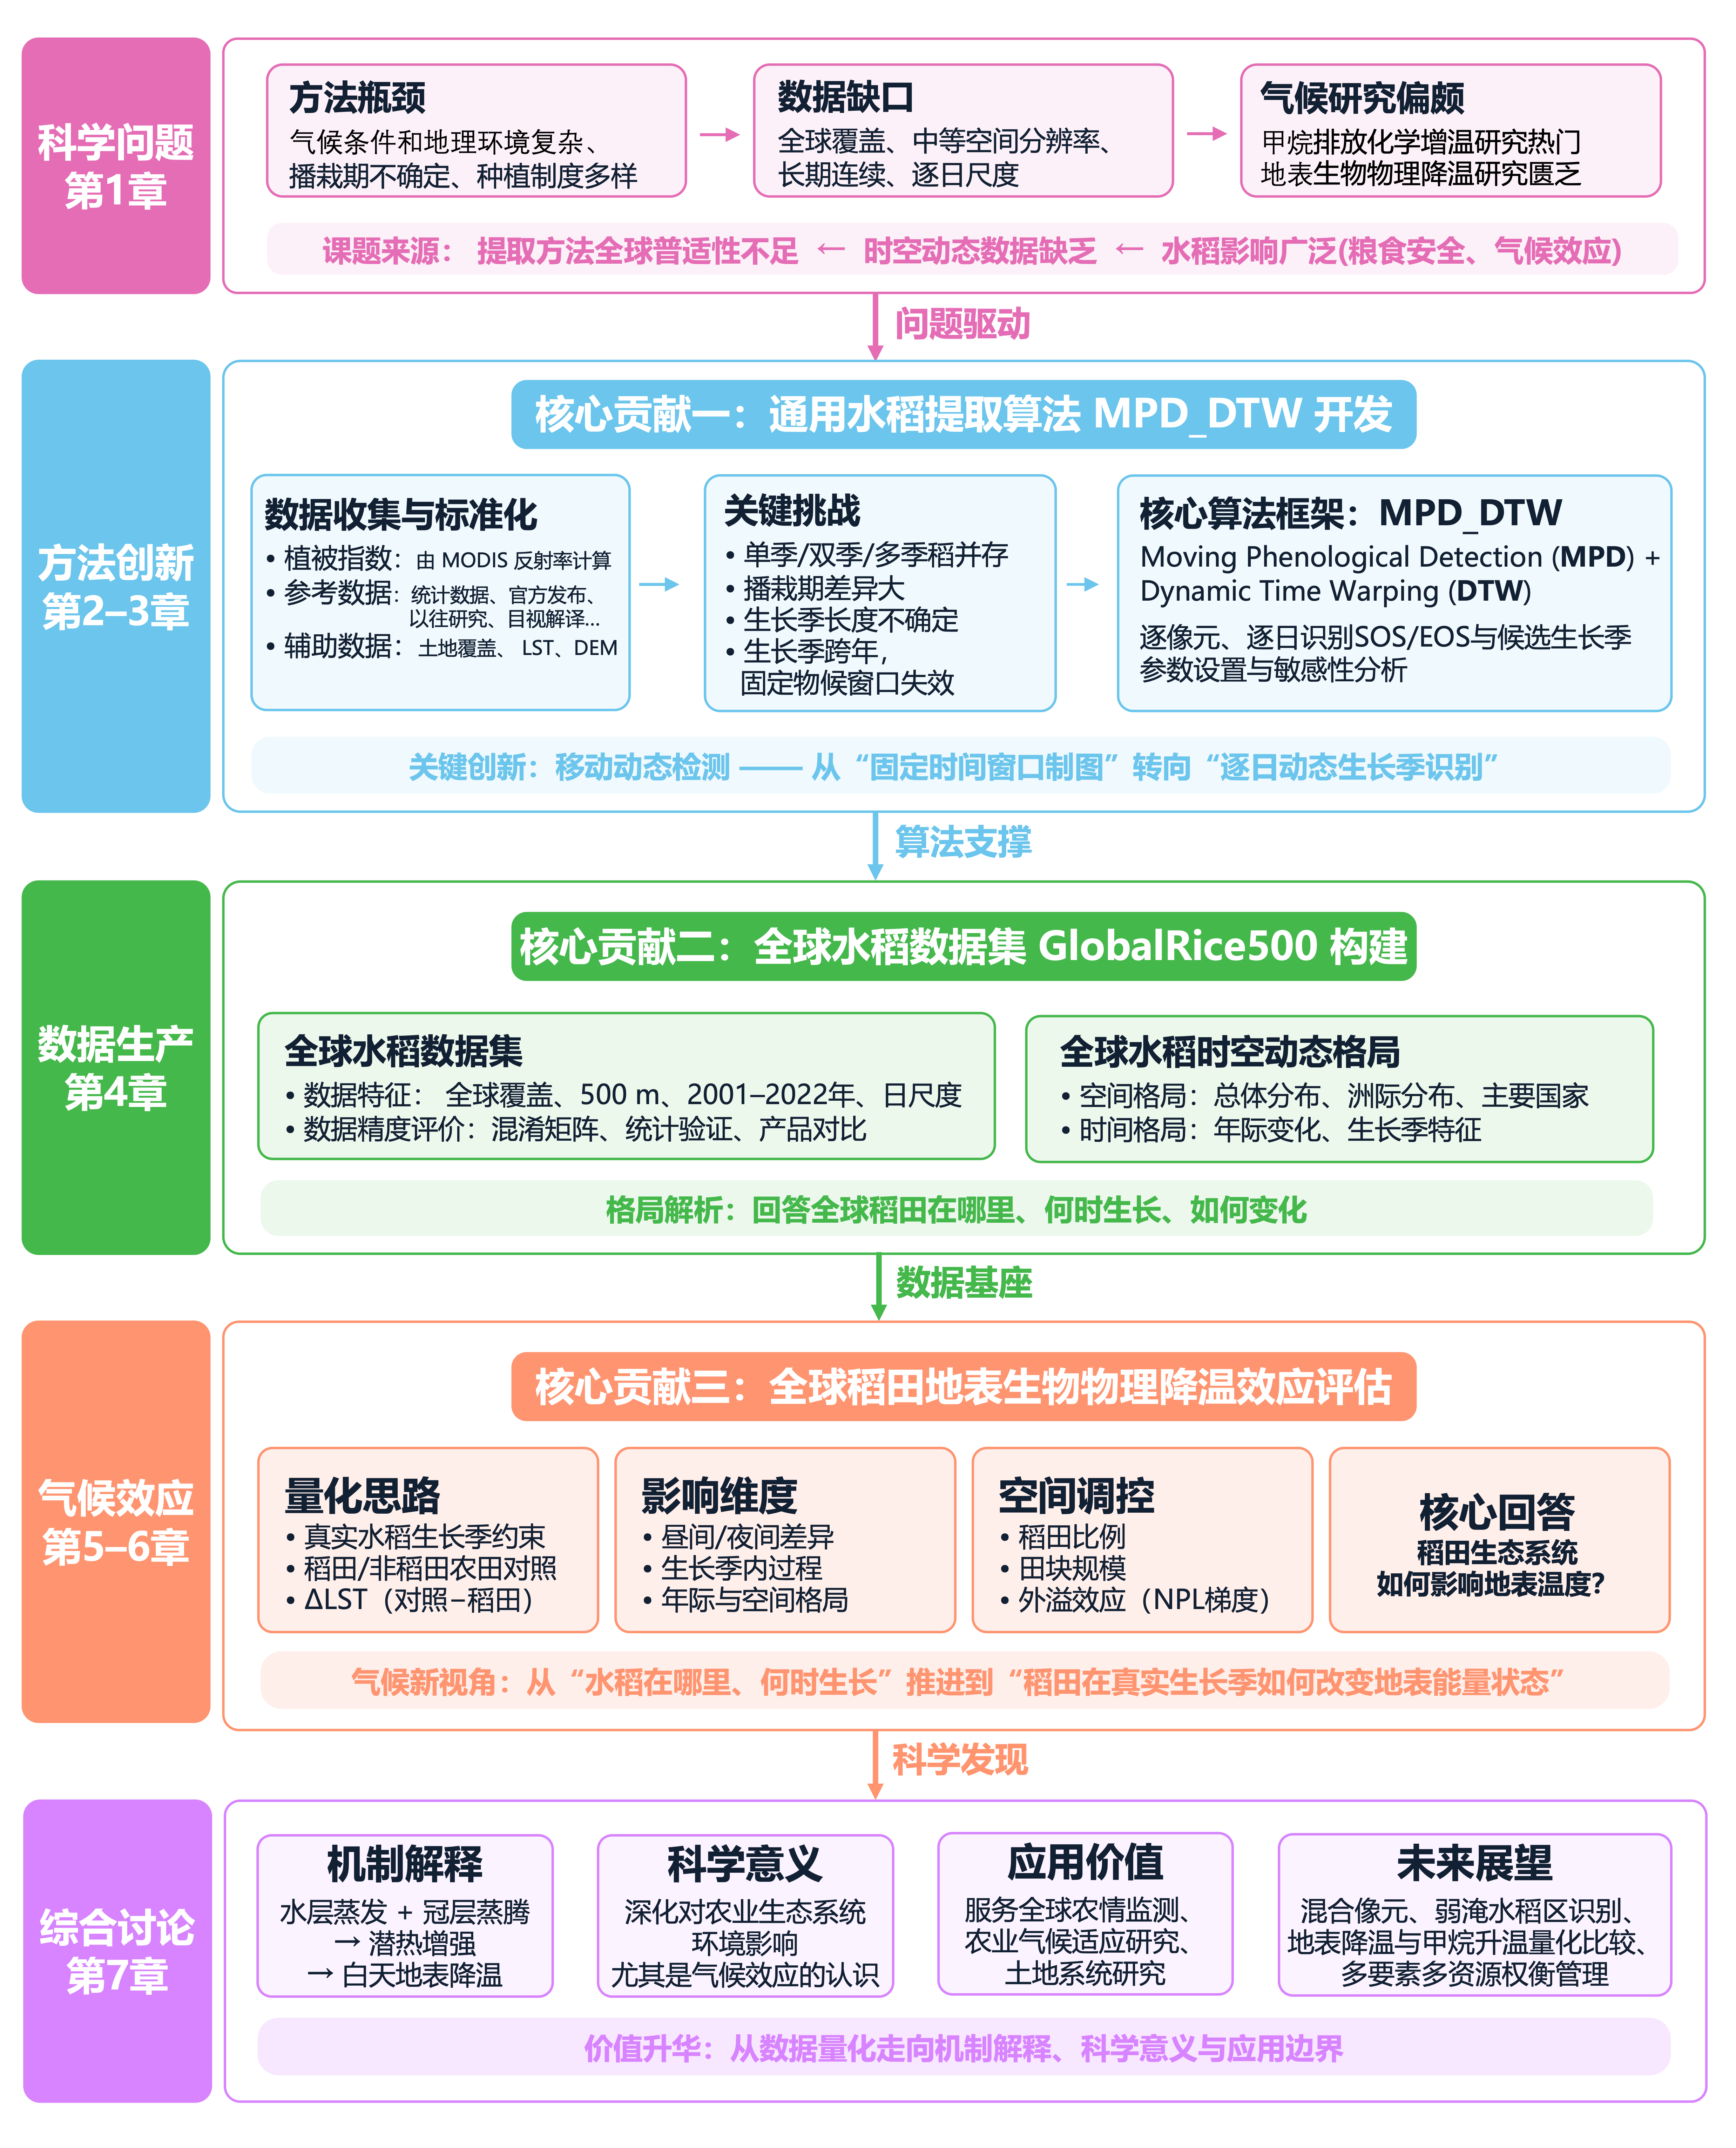
\includegraphics[width=0.95\linewidth]{figure/chapter1/overall_framework.png}
    \bicaption{本研究总体框架图}{Overall framework of this research}
    \label{fig:framework}
\end{figure}
